%%%%%%%%%%%%%%%%%%%%%%%%%%%%%%%%%%%%
% Header                           %
%%%%%%%%%%%%%%%%%%%%%%%%%%%%%%%%%%%%
% 
% Revisions: 2017-04-10 Martin R�del <martin.raedel@dlr.de>
%                       Initial draft
%               
% Contact:   Martin R�del,  martin.raedel@dlr.de
%            DLR Composite Structures and Adaptive Systems
%          
%                                 __/|__
%                                /_/_/_/  
%            www.dlr.de/fa/en      |/ DLR
%
%%%%%%%%%%%%%%%%%%%%%%%%%%%%%%%%%%%%
% Content                          %
%%%%%%%%%%%%%%%%%%%%%%%%%%%%%%%%%%%%

\chapter{Pre- and postprocessing with \texorpdfstring{\protect\marktool{\paraviewname}}{\paraviewname{}}}
\setcounter{currentlevel}{6}

\def\paraviewscreenshotwidthfac{0.8}

%%%%%%%%%%%%%%%%%%%%%%%%%%%%%%%%%%%%
% Header                           %
%%%%%%%%%%%%%%%%%%%%%%%%%%%%%%%%%%%%
% 
% Revisions: 2017-04-10 Martin R�del <martin.raedel@dlr.de>
%                       Initial draft
%               
% Contact:   Martin R�del,  martin.raedel@dlr.de
%            DLR Composite Structures and Adaptive Systems
%          
%                                 __/|__
%                                /_/_/_/  
%            www.dlr.de/fa/en      |/ DLR
% 
%%%%%%%%%%%%%%%%%%%%%%%%%%%%%%%%%%%%
% Content                          %
%%%%%%%%%%%%%%%%%%%%%%%%%%%%%%%%%%%%

\leveldown{Input \& Import}

\marktool{\toolname} creates result files in the \marktool{Exodus} format. This format can read by \marktool{\paraviewname}. It is basically the same format as the \marktool{\exodusname} finite element mesh discretization. Therefore, also the underlying \marktool{\exodusname} mesh can be visualized in \marktool{\paraviewname}.

If multiple processors are used for the execution of \marktool{\toolname} each MPI core creates an individual \marktool{Exodus} output file. The individual result files must be merged before the output can be used in \marktool{\paraviewname}. For the proper procedure please consult section \ref{sec:Peridigm:Run:Execution:Local:MergeOutput}.

To import a file to \marktool{\paraviewname} perform the following steps

\begin{enumerate}[noitemsep]
\item From the menu bar:
  \begin{itemize}[noitemsep]
  \item Click File
  \item Click Open
  \item Select the .g/.e-\marktool{\toolname} input or output file
  \end{itemize}
  or click 
\includegraphics[width=\iconsize]{Figures/Icons/pqOpen32} in the Main Controls toolbar
\item In the newly opened \textit{Properties} tab:
  \begin{itemize}[noitemsep]
  \item Choose the variables you want to use for post-processing
  \item Choose the blocks, assemblies and material regions you want to include
  \item Click \textit{Apply}
  \end{itemize}
\end{enumerate}

\newpage
%%%%%%%%%%%%%%%%%%%%%%%%%%%%%%%%%%%%
% Header                           %
%%%%%%%%%%%%%%%%%%%%%%%%%%%%%%%%%%%%
% 
% Revisions: 2017-04-10 Martin R�del <martin.raedel@dlr.de>
%                       Initial draft
%               
% Contact:   Martin R�del,  martin.raedel@dlr.de
%            DLR Composite Structures and Adaptive Systems
%          
%                                 __/|__
%                                /_/_/_/  
%            www.dlr.de/fa/en      |/ DLR
% 
%%%%%%%%%%%%%%%%%%%%%%%%%%%%%%%%%%%%
% Content                          %
%%%%%%%%%%%%%%%%%%%%%%%%%%%%%%%%%%%%

\levelstay{Result data}

\marktool{\paraviewname} distinguishes three types of result data:

\begin{multicols}{3}
\begin{itemize}
\addtolength\itemsep{-2ex}
 \item point data
 \item cell data
 \item field data
\end{itemize}
\end{multicols}

Point data is specified at each grid point. Cell data is specified per cell. Field data occurs for user-defined output values. Several linear and non-linear cell types currently exist for one-, two- or three-dimensional applications. E.g. a cell can be a quadrilateral between four nodes in two dimensions, a hexahedron volume between eight nodes in three dimensions or others. All cell types are shown in \cite{vtkfileformats}.

Following is a list of \marktool{\toolname} post-processing items and their classification as point data or cell data.

\begin{multicols}{2}
\begin{itemize}
\addtolength\itemsep{-2ex}
\item Point data results:
  \begin{itemize}
  \addtolength\itemsep{-2ex}
  \item Contact\_Force
  \item Displacement
  \item Force
  \item Global Node Ids
  \item Velocity
  \item $\ldots$
  \end{itemize}
\item Field data results:
  \begin{itemize}
  \addtolength\itemsep{-2ex}
  \item Compute Class Parameter results
  \end{itemize}
\columnbreak
\item Cell data results:
  \begin{itemize}
  \addtolength\itemsep{-2ex}
  \item Damage
  \item Dilatation
  \item Element\_Id
  \item Global Element Ids
  \item Number\_Of\_Neighbors
  \item Object IDs
  \item Proc\_num
  \item Radius
  \item Weighted\_Volume
  \item $\ldots$
  \end{itemize}
\end{itemize}
\end{multicols}

\newpage
%%%%%%%%%%%%%%%%%%%%%%%%%%%%%%%%%%%%
% Header                           %
%%%%%%%%%%%%%%%%%%%%%%%%%%%%%%%%%%%%
% 
% Revisions: 2017-04-10 Martin R�del <martin.raedel@dlr.de>
%                       Initial draft
%               
% Contact:   Martin R�del,  martin.raedel@dlr.de
%            DLR Composite Structures and Adaptive Systems
%          
%                                 __/|__
%                                /_/_/_/  
%            www.dlr.de/fa/en      |/ DLR
% 
%%%%%%%%%%%%%%%%%%%%%%%%%%%%%%%%%%%%
% Content                          %
%%%%%%%%%%%%%%%%%%%%%%%%%%%%%%%%%%%%

\levelstay{Selection}
\label{sec:Use_ParaView_Selection}

\leveldown{Create a selection}
\label{sec:Use_ParaView_Selection_Create}

Selections are

\begin{itemize}[noitemsep]
  \item a mechanism to identify subset of a dataset
  \item Focus on selected subset:
  \begin{itemize}[noitemsep]
    \item Inspect properties of the subset
    \item Further process subset alone
  \end{itemize}
  \item Track subset over time
\end{itemize}

Selections are performed in a toolbar in the RenderView. At first it has to be chosen if the items should be added to or removed from the selection using the following buttons:

\begin{tabularx}{\linewidth}{clXclXcl}

\includegraphics[width=\iconsize]{Figures/Icons/pqSelectPlus16}	& Add selection	&&

\includegraphics[width=\iconsize]{Figures/Icons/pqSelectMinus16}	& Subtract selection	&&

\includegraphics[width=\iconsize]{Figures/Icons/pqSelectToggle16}	& Toggle selection
\end{tabularx}

In a second step the kind of item, cells or points, to be selected has to be specified:

\begin{tabularx}{\linewidth}{lXclXcl}
Points: &&

\includegraphics[width=\iconsize]{Figures/Icons/pqSurfaceSelectionPoint24}	& Select points on	&&

\includegraphics[width=\iconsize]{Figures/Icons/pqFrustumSelectionPoint24}	& Select points through	\\
&&

\includegraphics[width=\iconsize]{Figures/Icons/pqPolygonSelectSurfacePoint24}	& Select points with polygon	&&

\includegraphics[width=\iconsize]{Figures/Icons/pqSurfaceSelectionPointInteractive}	& Select points interactive	\\
% 
Cells: &&

\includegraphics[width=\iconsize]{Figures/Icons/pqSurfaceSelectionCell24}	& Select cells on	&&

\includegraphics[width=\iconsize]{Figures/Icons/pqFrustumSelectionCell24}	& Select cells through	\\
&&

\includegraphics[width=\iconsize]{Figures/Icons/pqPolygonSelectSurfaceCell24.png}	& Select cells with polygon	&&

\includegraphics[width=\iconsize]{Figures/Icons/pqSurfaceSelectionCellInteractive}	& Select cells interactive
\end{tabularx}

Selection steps can be repeated as long as no Filter dependent on the selection is active. The currently selected entities are highlighted.

\levelstay{Limit display to selection}
\label{sec:Use_ParaView_Selection_LimitTo}

To limit the model to a user defined selection:

\begin{enumerate}[noitemsep]
\item Import result file to \marktool{\paraviewname}
\item Create a selection
\item From the menu bar:
  \begin{itemize}[noitemsep]
  \item Click Filters
  \item Click Data Analysis
  \item Click \textit{Extract Selection}
  \end{itemize}
  or click 
\includegraphics[width=\iconsize]{Figures/Icons/pqExtractSelection24} in the Data Analysis toolbar
\item Click \textit{Apply} in the newly opened Properties tab
\end{enumerate}

\levelstay{Remarks}

\begin{enumerate}[noitemsep]
   \item  Selected points lie in a virtual box. If the deformation of the model are to big, the points move outside the box and the allocation is lost. This might be an issue for plotting data. This can be solved by setting the deformation scaling to zero.
\end{enumerate}


\newpage
%%%%%%%%%%%%%%%%%%%%%%%%%%%%%%%%%%%%
% Header                           %
%%%%%%%%%%%%%%%%%%%%%%%%%%%%%%%%%%%%
% 
% Revisions: 2017-04-10 Martin R�del <martin.raedel@dlr.de>
%                       Initial draft
%               
% Contact:   Martin R�del,  martin.raedel@dlr.de
%            DLR Composite Structures and Adaptive Systems
%          
%                                 __/|__
%                                /_/_/_/  
%            www.dlr.de/fa/en      |/ DLR
% 
%%%%%%%%%%%%%%%%%%%%%%%%%%%%%%%%%%%%
% Content                          %
%%%%%%%%%%%%%%%%%%%%%%%%%%%%%%%%%%%%

\levelup{View \& Display}
%%%%%%%%%%%%%%%%%%%%%%%%%%%%%%%%%%%%
% Header                           %
%%%%%%%%%%%%%%%%%%%%%%%%%%%%%%%%%%%%
% 
% Revisions: 2017-04-10 Martin R�del <martin.raedel@dlr.de>
%                       Initial draft
%               
% Contact:   Martin R�del,  martin.raedel@dlr.de
%            DLR Composite Structures and Adaptive Systems
%          
%                                 __/|__
%                                /_/_/_/  
%            www.dlr.de/fa/en      |/ DLR
% 
%%%%%%%%%%%%%%%%%%%%%%%%%%%%%%%%%%%%
% Content                          %
%%%%%%%%%%%%%%%%%%%%%%%%%%%%%%%%%%%%

\leveldown{Save view}
\label{sec:Paraview:View:Save}

To save a view configuration click an the \textit{Adjust Camera} button 
\includegraphics[width=\iconsize]{Figures/Icons/pqEditCamera16.png} in the icon bar of your \textit{RenderView}.
%%%%%%%%%%%%%%%%%%%%%%%%%%%%%%%%%%%%
% Header                           %
%%%%%%%%%%%%%%%%%%%%%%%%%%%%%%%%%%%%
% 
% Revisions: 2017-04-10 Martin R�del <martin.raedel@dlr.de>
%                       Initial draft
%               
% Contact:   Martin R�del,  martin.raedel@dlr.de
%            DLR Composite Structures and Adaptive Systems
%          
%                                 __/|__
%                                /_/_/_/  
%            www.dlr.de/fa/en      |/ DLR
%
%%%%%%%%%%%%%%%%%%%%%%%%%%%%%%%%%%%%
% Content                          %
%%%%%%%%%%%%%%%%%%%%%%%%%%%%%%%%%%%%

\levelstay{Display point/node numbers}
\label{sec:Paraview:Display:Point:Labels}

After importing the model it might be of interest to get the node/point numbers for the whole model or a specific selection. To show these numbers after importing the model:

\begin{enumerate}[noitemsep]
  \item Generate and extract the selection of interest according to \autoref{sec:Use_ParaView_Selection}
  \item Left-click on the imported model (set the model active)
  \item From the menubar:
    \begin{itemize}[noitemsep]
      \item Click \textit{View}
      \item Click \textit{Selection Display Inspector}
    \end{itemize}
  \item In the \textit{Selection Display Inspector} window:
    \begin{itemize}[noitemsep]
      \item Click on \textit{Point Labels}
      \item Select \textit{ID}
    \end{itemize}
  \item The point/node numbers appear as labels
\end{enumerate}

\begin{figure}[htbp]
\centering
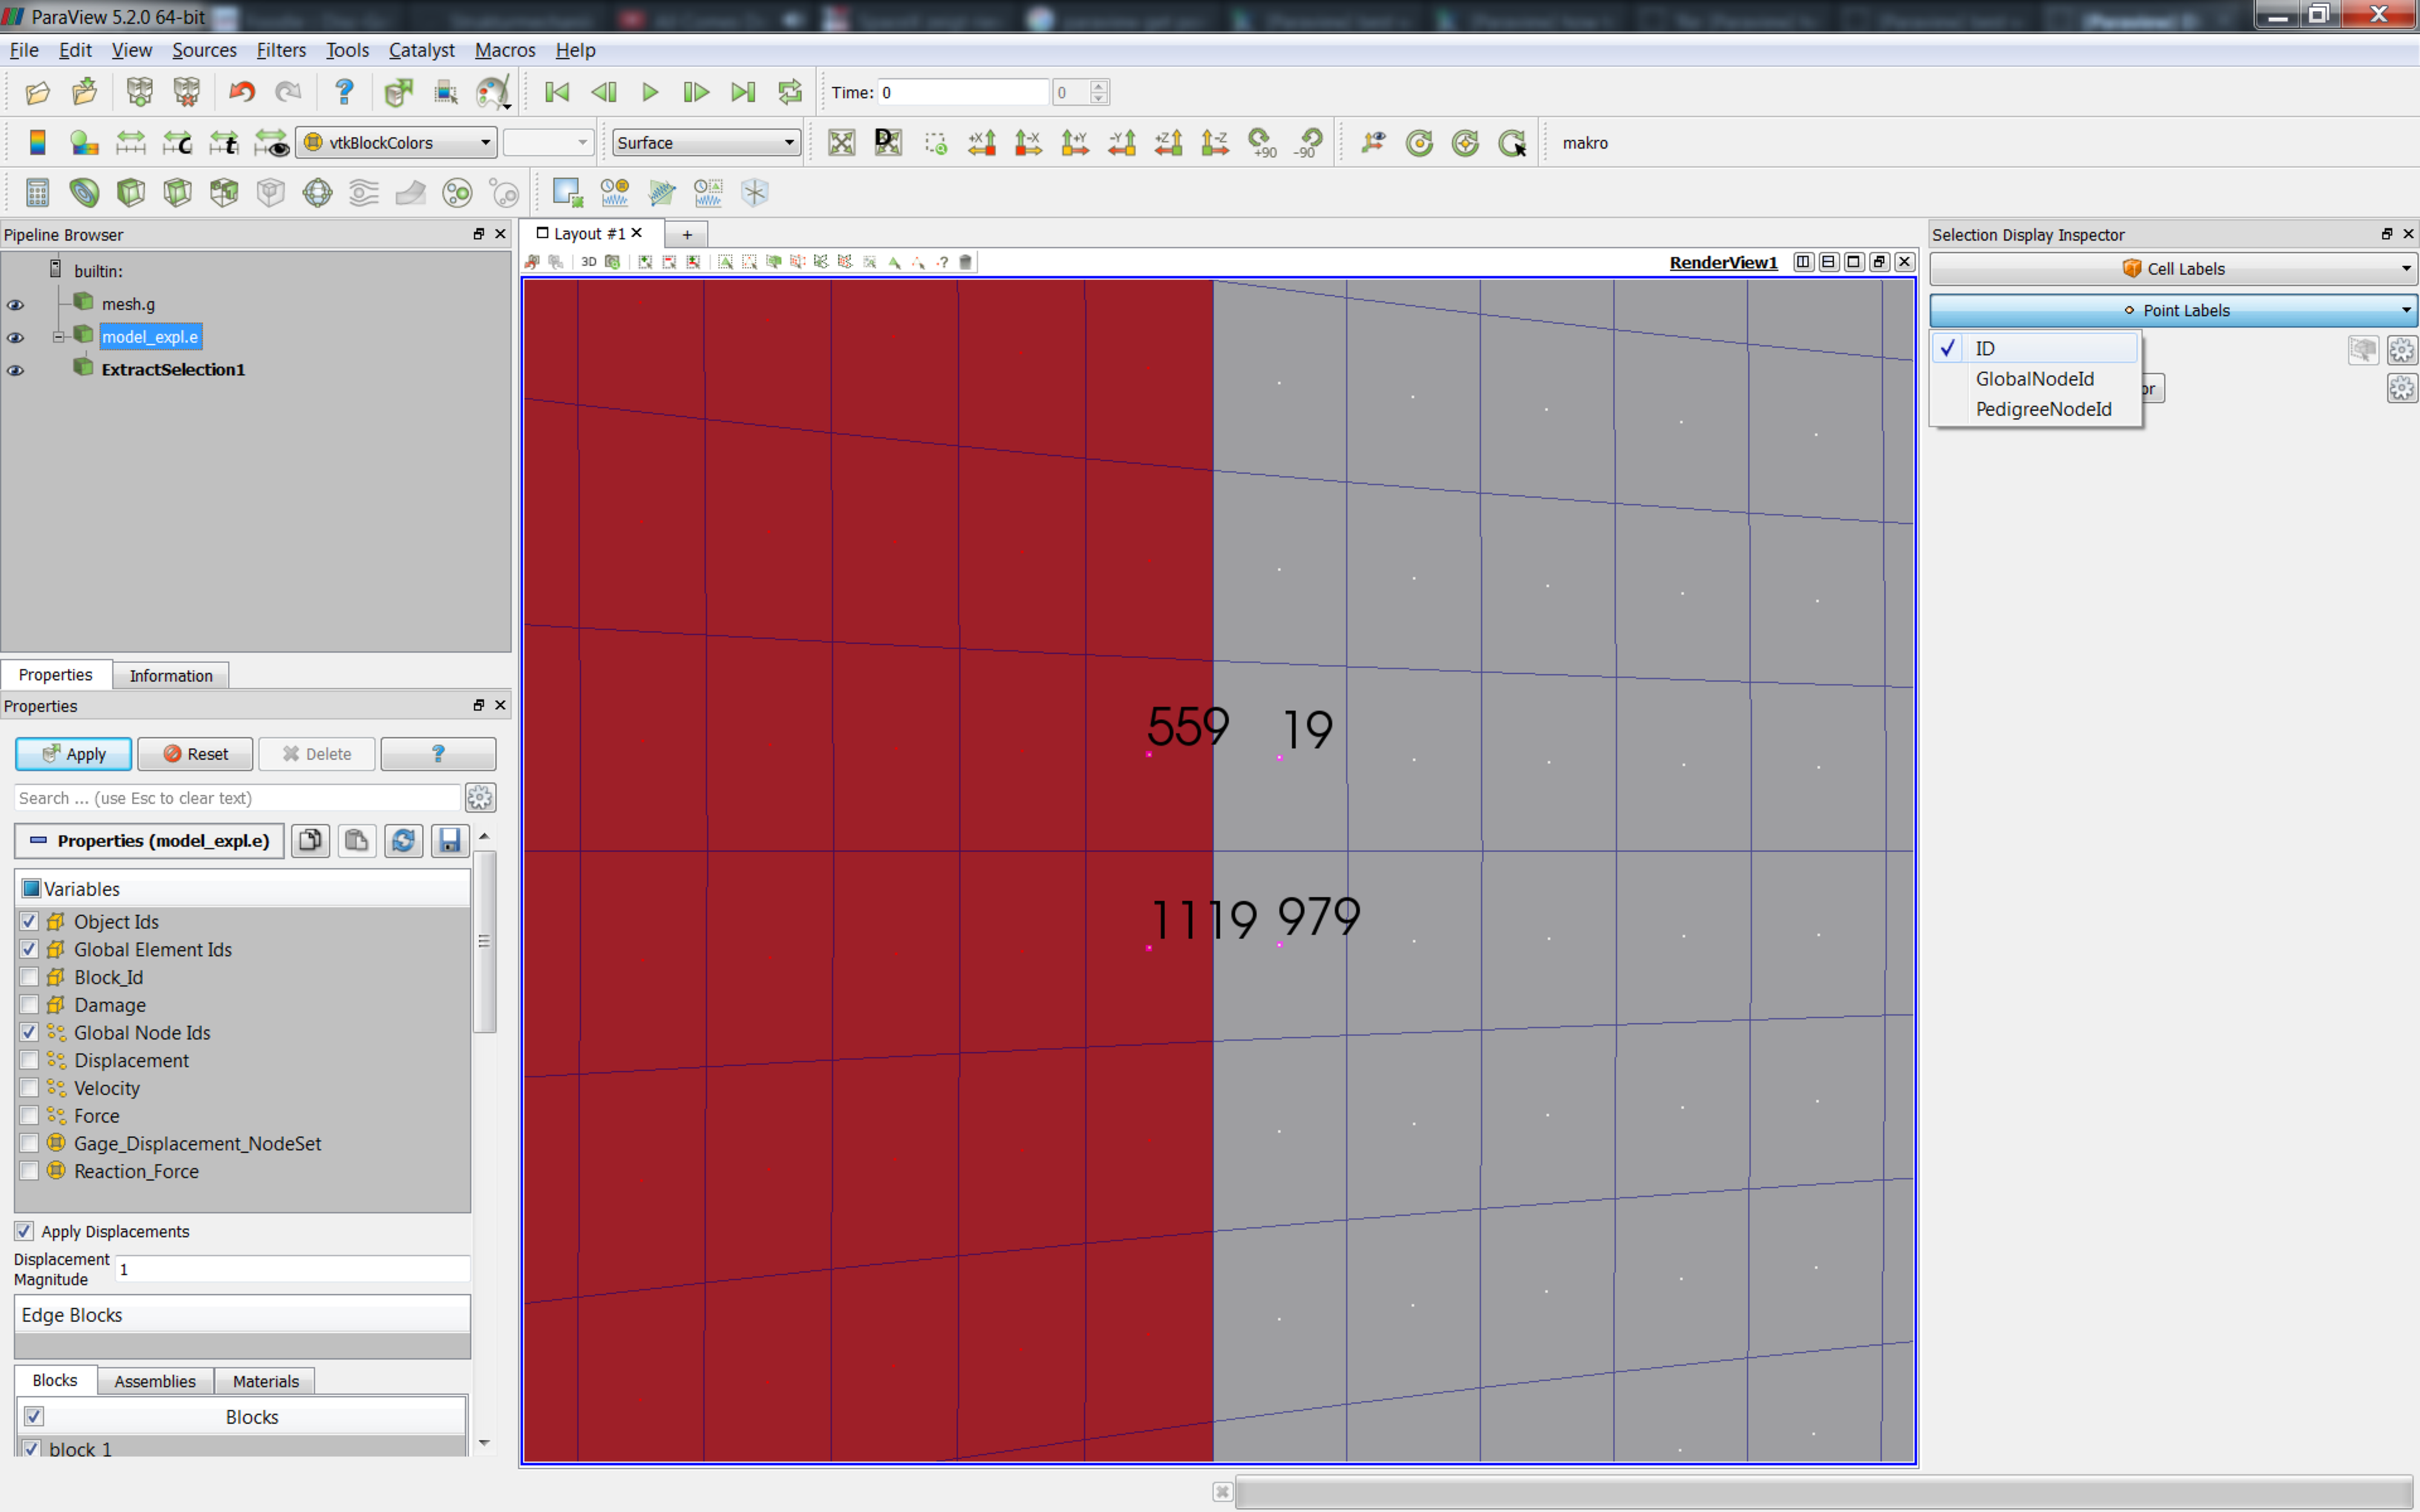
\includegraphics[width=\paraviewscreenshotwidthfac\linewidth]{Figures/Screenshots/ParaView_Display_NodeLabels}
\caption{Display of selection point/node numbers}
\label{fig:Use_ParaView_Display_NodeLabels}
\end{figure}

%%%%%%%%%%%%%%%%%%%%%%%%%%%%%%%%%%%%
% Header                           %
%%%%%%%%%%%%%%%%%%%%%%%%%%%%%%%%%%%%
% 
% Revisions: 2017-04-10 Martin R�del <martin.raedel@dlr.de>
%                       Initial draft
%               
% Contact:   Martin R�del,  martin.raedel@dlr.de
%            DLR Composite Structures and Adaptive Systems
%          
%                                 __/|__
%                                /_/_/_/  
%            www.dlr.de/fa/en      |/ DLR
% 
%%%%%%%%%%%%%%%%%%%%%%%%%%%%%%%%%%%%
% Content                          %
%%%%%%%%%%%%%%%%%%%%%%%%%%%%%%%%%%%%

\levelstay{Visualize nodesets}

To visualize the nodesets from a \marktool{\exodusname} mesh or \marktool{\toolname} results file in \marktool{\paraviewname} perform the following steps

\begin{enumerate}[noitemsep]
\item From the menu bar: \label{itm:Use_ParaView_Visualize_NoseSet_Step1}
  \begin{itemize}[noitemsep]
  \item Click File
  \item Click Open
  \item Select the .g/.e-\marktool{\toolname} input or output file
  \end{itemize}
  or click 
\includegraphics[width=\iconsize]{Figures/Icons/pqOpen32} in the Main Controls toolbar
\item In the newly opened \textit{Properties} tab:
  \begin{itemize}[noitemsep]
  \item Click the gear symbol 
\includegraphics[width=\iconsize]{Figures/Icons/pqAdvanced26} next to the \textit{Search} line
  \item \textit{Sets} and \textit{Maps} tables become available for selection
  \item Select the nodesets to display
  \item Unselect all Blocks
  \item Click \textit{Apply}
  \end{itemize}
\item Create a \textit{Glyph} based on the current model as described in \autoref{sec:ParaView_Damage_Plots_on_Nodes_as_Spheres} (without the result data stuff of course)
\item Repeat step \ref{itm:Use_ParaView_Visualize_NoseSet_Step1}
\item In the newly opened \textit{Properties} tab:
  \begin{itemize}[noitemsep]
  \item Select all Blocks
  \item Set the \textit{Opacity} to 0.4
  \item Click \textit{Apply}
  \end{itemize}
\end{enumerate}

Similarly, the nodesets in the peridynamic collocation point translation can be visualized. The following figure shows the base \marktool{\exodusname} finite element mesh in gray. Superimposed with the finite element mesh are the nodes of a finite element nodeset (blue) and the nodeset in the peridynamic translation (green).

\begin{figure}[htbp]
\centering
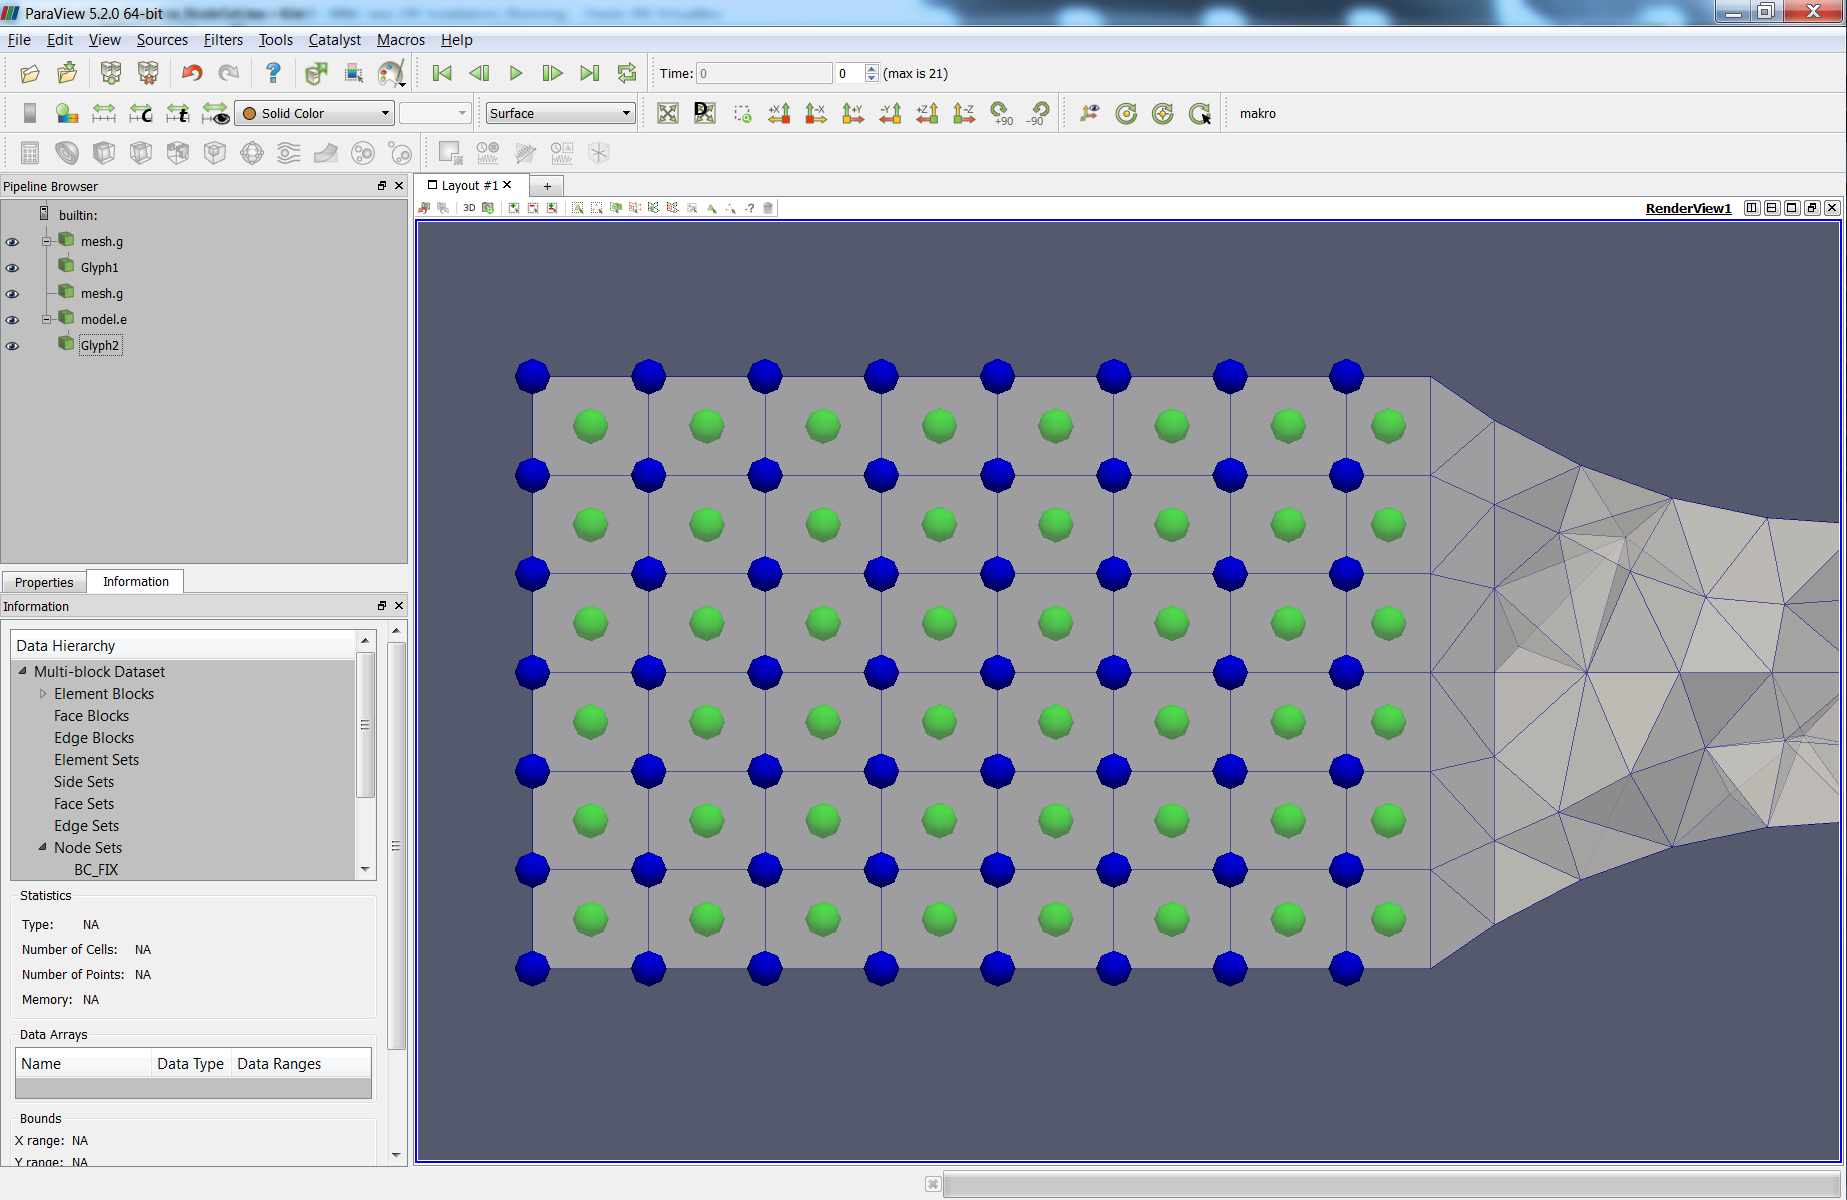
\includegraphics[width=\paraviewscreenshotwidthfac\linewidth]{Figures/Screenshots/ParaView_Visualize_NodeSets}
\caption{Visualization of base finite element mesh (gray), finite element nodeset (blue) and nodeset after transformation to peridynamic collocation points (green)}
\label{fig:Use_ParaView_Visualize_NoseSets}
\end{figure}

\FloatBarrier
%%%%%%%%%%%%%%%%%%%%%%%%%%%%%%%%%%%%
% Header                           %
%%%%%%%%%%%%%%%%%%%%%%%%%%%%%%%%%%%%
% 
% Revisions: 2017-04-10 Martin R�del <martin.raedel@dlr.de>
%                       Initial draft
%               
% Contact:   Martin R�del,  martin.raedel@dlr.de
%            DLR Composite Structures and Adaptive Systems
%          
%                                 __/|__
%                                /_/_/_/  
%            www.dlr.de/fa/en      |/ DLR
% 
%%%%%%%%%%%%%%%%%%%%%%%%%%%%%%%%%%%%
% Content                          %
%%%%%%%%%%%%%%%%%%%%%%%%%%%%%%%%%%%%

\levelstay{Damage plot on nodes as spheres}
\label{sec:ParaView_Damage_Plots_on_Nodes_as_Spheres}

Commonly, the \marktool{\toolname} results are plotted on so called \texttt{Glyphs} in \marktool{\paraviewname}. A \texttt{Glyph} is a geometric object with a specific size, a direction and a color, which is drawn at certain positions within the vector field. \texttt{Glyph} shapes can be an

\begin{multicols}{4}
\begin{itemize}
\addtolength\itemsep{-2ex}
\item Arrow
\item Cone
\item Box
\item Cylinder
\item Line
\item Sphere
\item 2D glyph
\end{itemize}
\end{multicols}

A natural choice for peridynamic nodes is the sphere. Unfortunately, cell data can not be plotted directly in a \texttt{Glyph} plot. Therefore, the cell data has to be converted to point data first.

\begin{enumerate}[noitemsep]
\item Import result file to \marktool{\paraviewname}
\item Left-click on the result file once in the Pipeline Browser (mark the result file)
\item From the menu bar:
  \begin{itemize}[noitemsep]
  \item Click Filters
  \item Click Alphabetical
  \item Click \textit{Cell Data to Point Data}
  \end{itemize}
\item Left-click on the new item \textit{Cell Data to Point Data} in the Pipeline Browser
\item From the menu bar:
  \begin{itemize}[noitemsep]
  \item Click Filters
  \item Click Common
  \item Click \textit{Glyph}
  \end{itemize}
  or choose the \textit{Glyph}-symbol from the common filter icon toolbar
\item In the \textit{Glyph} properties window choose:
  \begin{itemize}[noitemsep]
  \item Glyph Type:	\tab \textit{Sphere}
  \item Scalars:	\tab \textit{Damage}
  \item Vectors:	\tab \textit{Displacement}
  \item Scale factor:	\tab Choose according to your needs
  \item Glyph mode:	\tab \textit{All Points}
  \item Coloring:	\tab \textit{Damage}
  \end{itemize}
  and click \textit{Apply}
\item Afterwards, return to the properties window, go to the \texttt{Display} section and choose:
  \begin{itemize}[noitemsep]
  \item Representation:	\tab \textit{Surface}
  \item Coloring:	\tab \textit{Damage}
  \end{itemize}
\end{enumerate}

Afterwards, you can skip through the time steps of your analysis in the Current Time Controls toolbar. It maybe necessary to adjust the range of the legend to the current time step minimum or maximum.

\newpage
%%%%%%%%%%%%%%%%%%%%%%%%%%%%%%%%%%%%
% Header                           %
%%%%%%%%%%%%%%%%%%%%%%%%%%%%%%%%%%%%
% 
% Revisions: 2017-04-10 Martin R�del <martin.raedel@dlr.de>
%                       Initial draft
%               
% Contact:   Martin R�del,  martin.raedel@dlr.de
%            DLR Composite Structures and Adaptive Systems
%          
%                                 __/|__
%                                /_/_/_/  
%            www.dlr.de/fa/en      |/ DLR
% 
%%%%%%%%%%%%%%%%%%%%%%%%%%%%%%%%%%%%
% Content                          %
%%%%%%%%%%%%%%%%%%%%%%%%%%%%%%%%%%%%

\levelup{Plotting}

%%%%%%%%%%%%%%%%%%%%%%%%%%%%%%%%%%%%
% Header                           %
%%%%%%%%%%%%%%%%%%%%%%%%%%%%%%%%%%%%
% 
% Revisions: 2017-04-10 Martin R�del <martin.raedel@dlr.de>
%                       Initial draft
%               
% Contact:   Martin R�del,  martin.raedel@dlr.de
%            DLR Composite Structures and Adaptive Systems
%          
%                                 __/|__
%                                /_/_/_/  
%            www.dlr.de/fa/en      |/ DLR
%
%%%%%%%%%%%%%%%%%%%%%%%%%%%%%%%%%%%%
% Content                          %
%%%%%%%%%%%%%%%%%%%%%%%%%%%%%%%%%%%%

\leveldown{Plot selection data over time}

To plot selection data, e.g. point results, over calculation time perform the following steps:

\begin{enumerate}[noitemsep]
\item Import result file to \marktool{\paraviewname}
\item Create a selection, e.g. to a single or two points
\item From the menu bar:
  \begin{itemize}[noitemsep]
  \item Click Filters
  \item Click Data Analysis
  \item Click \textit{Plot Selection Over Time}
  \end{itemize}
  or click 
\includegraphics[width=\iconsize]{Figures/Icons/pqPlotSelectionOverTime24} in the Data Analysis toolbar
\item In the newly opened Properties tab:
  \begin{itemize}[noitemsep]
  \item Review the Copied Selection
  \item Click \textit{Apply}
  \item Let \marktool{\paraviewname} process your request a couple of seconds
  \item For the actual values deselect the \textit{Only Report Selection Statistics} checkbox
  \item Click \textit{Apply}
  \item Wait until the progressbar in the bottom right is completed
  \item Select from the selection entities the items you are currently interested in
  \item Choose the \textit{Series Parameters} you are interested in (there is the same quantity for each selection entity, so a couple of times if you have multiple entities in your selection, choose wisely)
  \item Your requested values should show up in the \textit{QuartileChartView}
  \end{itemize}
\item You can skip through the time steps of your analysis in the Current Time Controls toolbar. The current time is shown as the vertical bar in the chart view
\end{enumerate}

To see the actual values in a spreadsheet:

\begin{enumerate}[noitemsep]
\item Right-click on the QuartileChartView top line (where e.g. QuartileChartView1 stands)
\item Create a selection, e.g. to a single or two points
\item Select:
  \begin{itemize}[noitemsep]
  \item Convert To ...
  \item Spreadsheet view
  \end{itemize}
\item In case you want to return to the Chart View you can do so accordingly but you have to repeat the data selection steps mentioned above
\end{enumerate}

A combined view:

\begin{figure}[htbp]
\centering
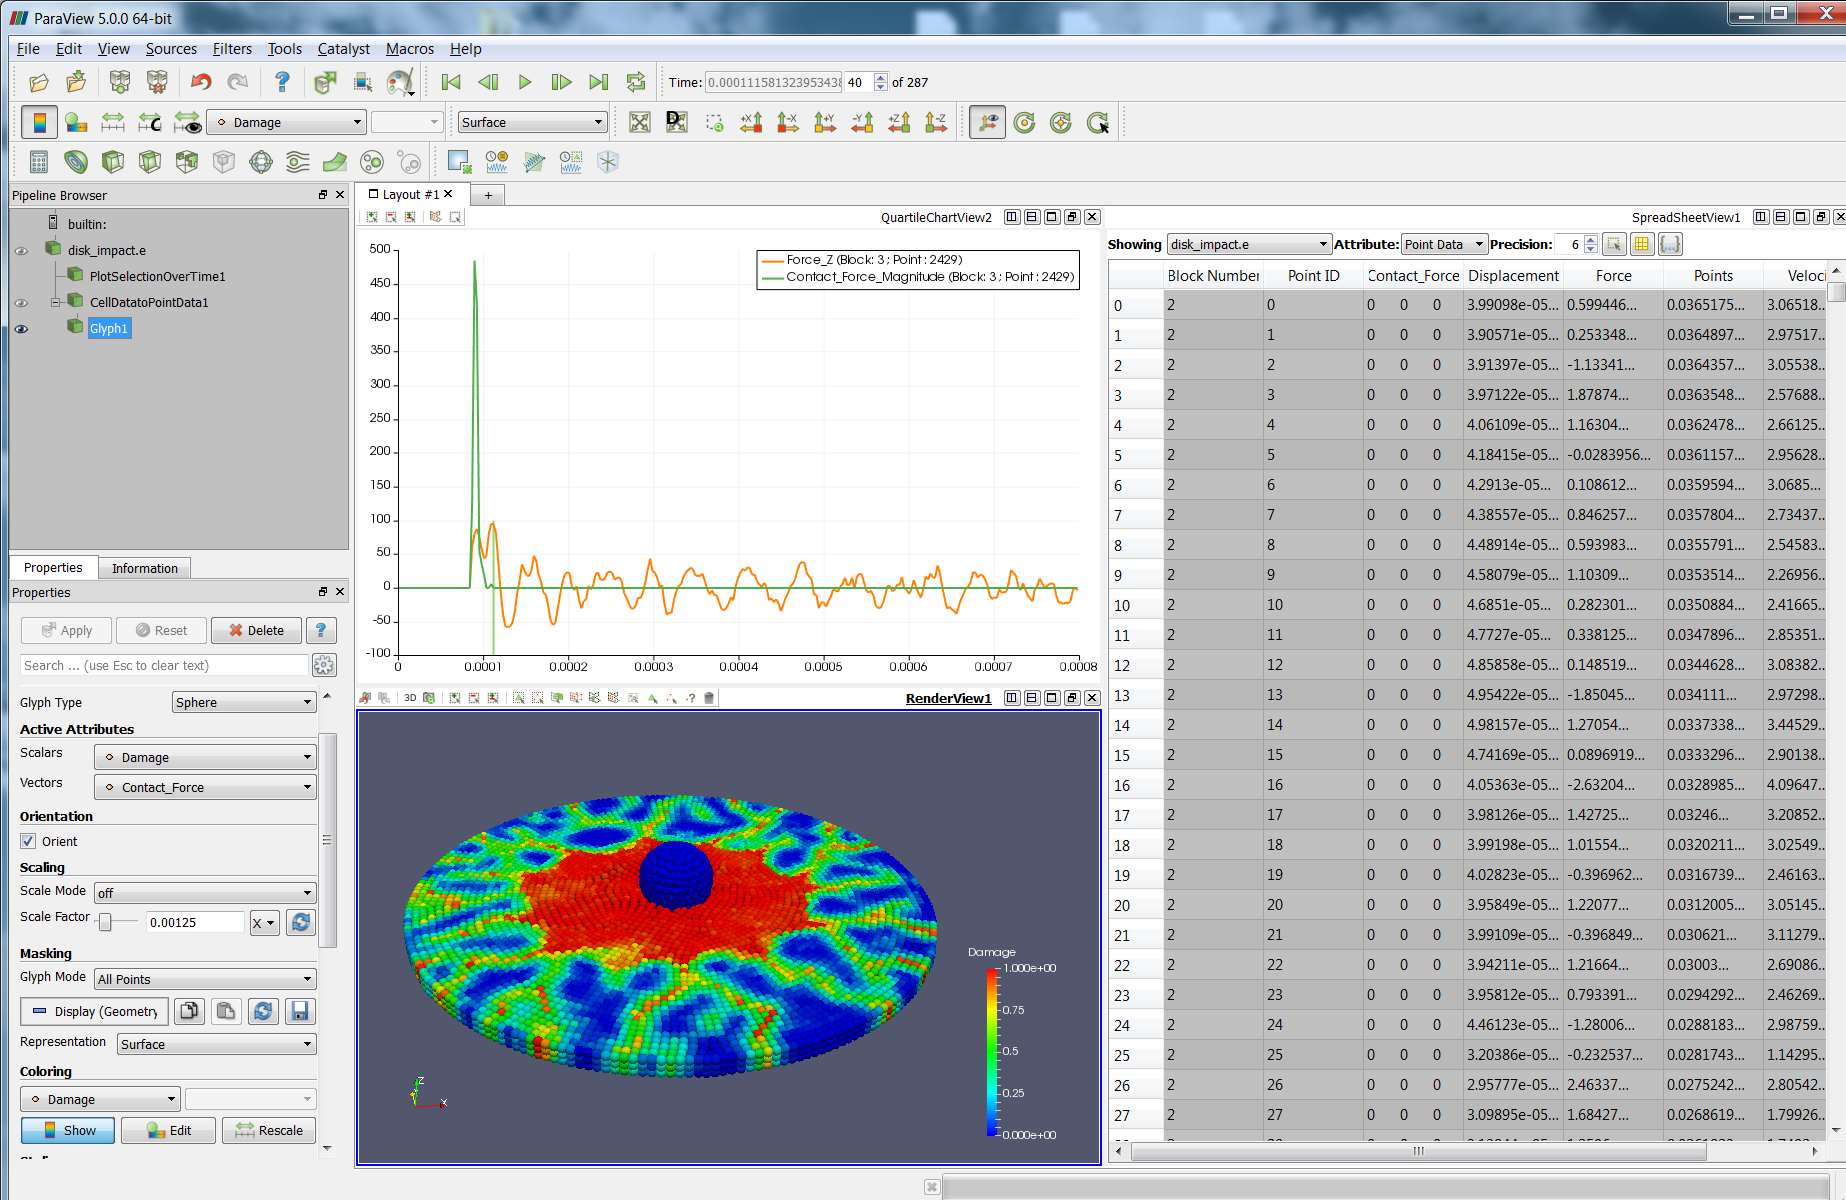
\includegraphics[width=\paraviewscreenshotwidthfac\linewidth]{Figures/Screenshots/State_ChartView_Combined}
\caption{Combined \marktool{\paraviewname} view}
\label{fig:Combined_ParaView_view}
\end{figure}

To save the data for plotting in \verb+pgfplots+:

\begin{enumerate}[noitemsep]
\item Select the PlotOverSelection in the \textit{Pipeline Browser} or left click in the ChartView or SpreadsheetView
\item From the menu bar:
  \begin{itemize}[noitemsep]
  \item Click File
  \item Click Save Data
  \end{itemize}
  or click 
\includegraphics[width=\iconsize]{Figures/Icons/pqSave32} in the Main Controls toolbar
\item Select folder and filename
\item Select csv file type
\item Click \textit{Ok}
\end{enumerate}

Beware, an individual csv-file is written for each and every entity in your selection. The file does not include any information on the entity ID or name. Thus, a sequential save-process for each single individual entity is advised. After each save, rename the resulting file.
%%%%%%%%%%%%%%%%%%%%%%%%%%%%%%%%%%%%
% Header                           %
%%%%%%%%%%%%%%%%%%%%%%%%%%%%%%%%%%%%
% 
% Revisions: 2017-04-10 Martin R�del <martin.raedel@dlr.de>
%                       Initial draft
%               
% Contact:   Martin R�del,  martin.raedel@dlr.de
%            DLR Composite Structures and Adaptive Systems
%          
%                                 __/|__
%                                /_/_/_/  
%            www.dlr.de/fa/en      |/ DLR
% 
%%%%%%%%%%%%%%%%%%%%%%%%%%%%%%%%%%%%
% Content                          %
%%%%%%%%%%%%%%%%%%%%%%%%%%%%%%%%%%%%

\levelstay{Force-displacement-plots}

\leveldown{General}

This plot shows the course of the ``nodal'' force in a constrained region of the model over the displacement of a discrete point. The sum of the forces is used as a representative of the integral force value a load cell would show. For the displacement the value of a discrete node or collocation point is used as a representative for the scalar value of an extensiometer or the machine displacement value.

\levelstay{\protect\toolname/\protect\paraviewname}

\leveldown{Requisition of output values in \protect\toolname}

To acquire forces and displacements for a defined part of a model \texttt{Compute Class Parameters} are used in \toolname. They are described in sections \ref{sec:Peridigm:QRG:ComputeClassParameters:Nodeset}, \ref{sec:Peridigm:QRG:ComputeClassParameters:Block} \& \ref{sec:Peridigm:QRG:ComputeClassParameters:NearestPoint}. The forces are requested for the node set or block where a body load or in this case boundary condition is applied on. The displacement is written for one point in this node set using the nearest neighbor approach to a defined spatial coordinate in the node set region. The initial position of the point the displacements are written for is also requested for convenience and checks.

\begin{code}
Compute Class Parameters
  Strain Gage Initial Position
    Compute Class "Nearest_Point_Data"
    X 0.0317
    Y 1.238
    Z 0.0
    Variable "Model_Coordinates"
    Output Label "Gage_Initial_Position"
    Verbose "True"
  Strain Gage Displacement
    Compute Class "Nearest_Point_Data"
    X 0.0317
    Y 1.238
    Z 0.0
    Variable "Displacement"
    Output Label "Gage_Displacement"
    Verbose "True"
  Reaction Force
    Compute Class "Node_Set_Data"
    Calculation Type "Sum"
    Node Set "bc_load"
    Variable "Force"
    Output Label "Reaction_Force"
\end{code}

Alternatively, it should also be possible to request the displacement for the same node set as the force and simply choose ``Minimum'' or ``Maximum'' as \textit{Calculation type}. This way, it is not required to adjust the spatial coordinates as in \textit{Compute Class ``Nearest\_Point\_Data''}. This works fine for a test case.

Additionally the global output variable types \textit{Displacement} and \textit{Force} must be requested in the output section.

\begin{code}
Output
  Output File Type "ExodusII"
  Output Filename "model"
  Output Frequency 1
  Output Variables
    ...
    Displacement "true"
    ...
    Force "true"
    ...
    Gage_Initial_Position "true"
    Gage_Displacement "true"
    Reaction_Force "true"
\end{code}

\levelstay{Access result data in \protect\paraviewname}

\begin{figure}[htbp]
\centering
  \begin{subfigure}{0.49\linewidth}
    \centering
    \begin{tikzpicture}
      % External figure
      \node[anchor=south west,inner sep=0] (image) at (0,0) {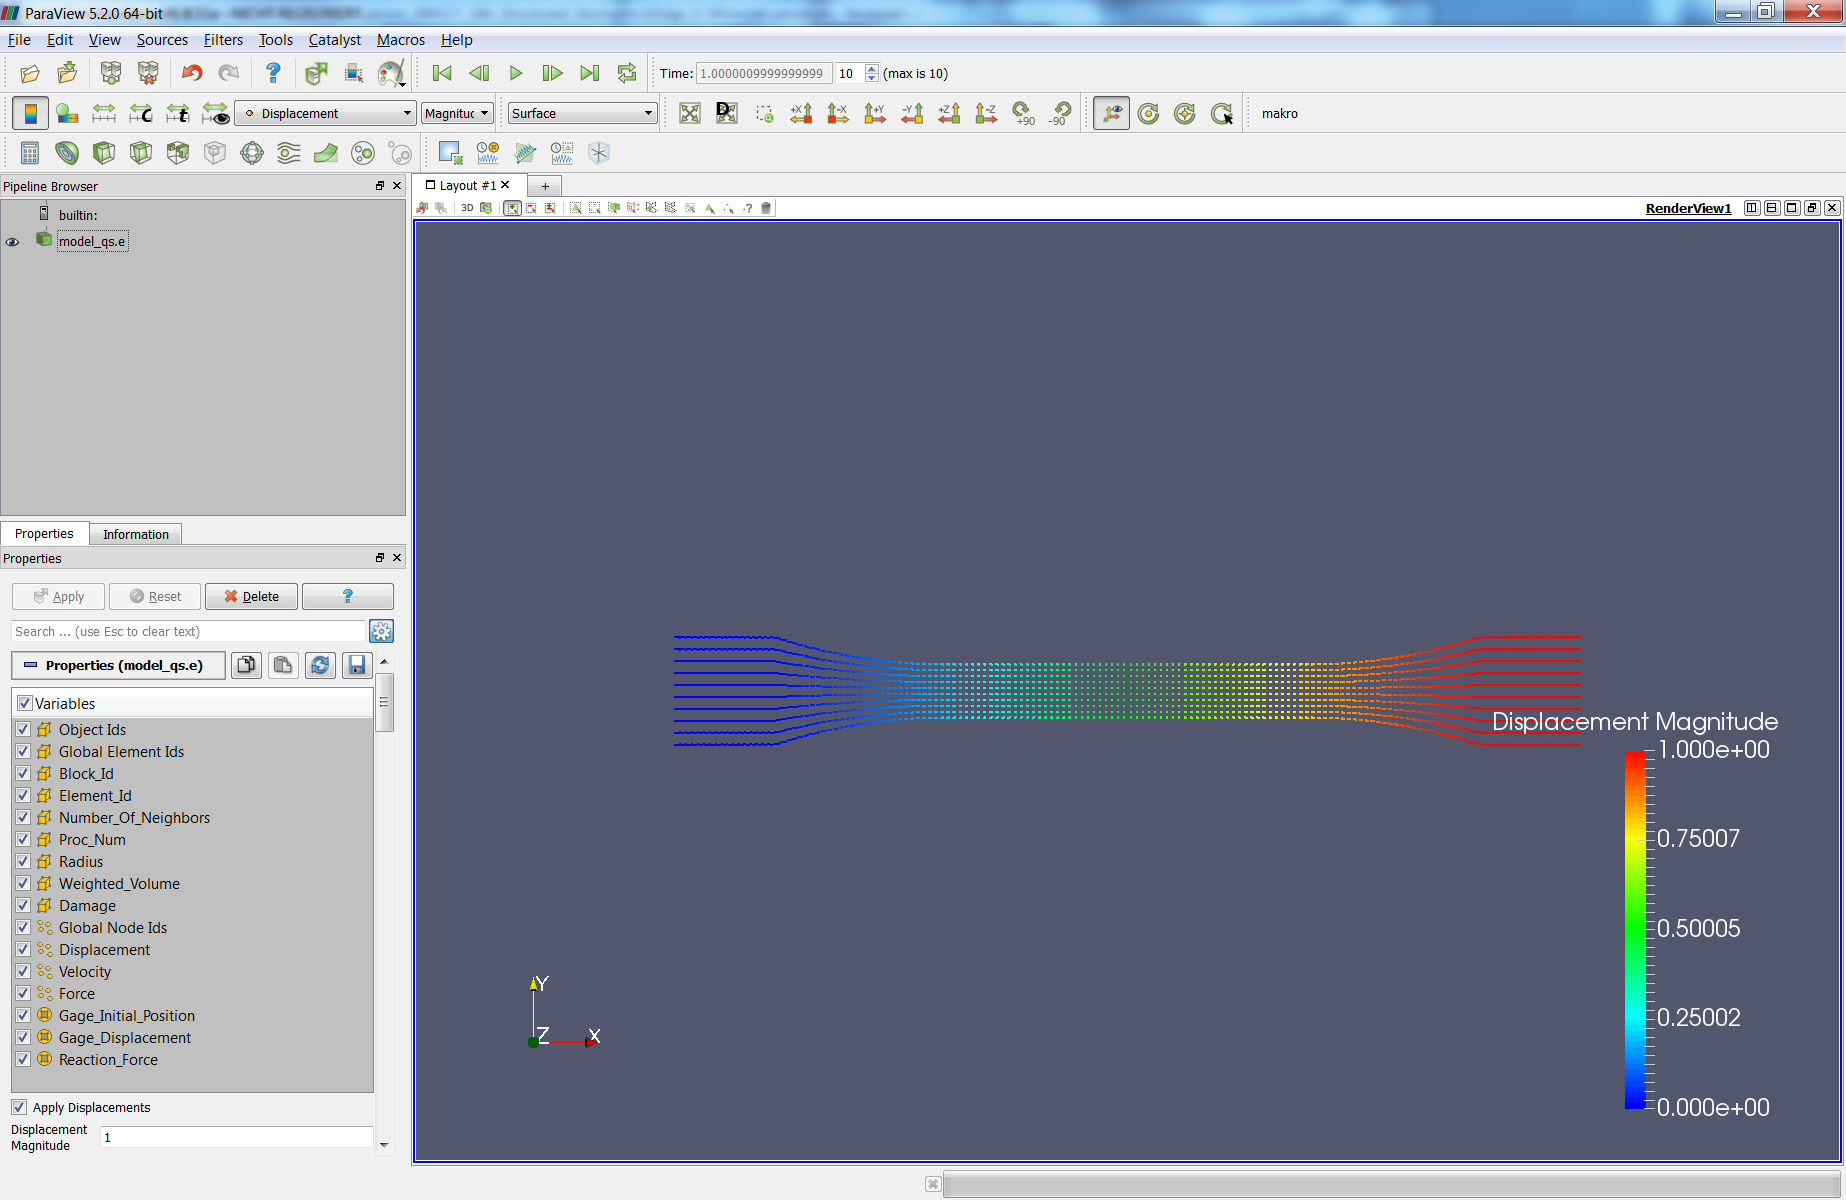
\includegraphics[width=\linewidth]{Figures/Screenshots/ParaView_ComputeClassParameter_ResultsData_1}};
      \begin{scope}[
        x={(image.south east)},
        y={(image.north west)},
      ]
        % Some label
        \node[fit={(0.007,0.10) (0.18,0.17)},myrectangularmarkup] (rect1) {};
        \node[anchor=west,mymarkuptext] (rect1label) at (rect1.east) {1};
        %
        \node[fit={(0.280,0.83) (0.31,0.86)},myrectangularmarkup] (rect2) {};
        \node[anchor=west,mymarkuptext] (rect2label) at (rect2.east) {2};
        % Help grid and labels
        %\pic{myimagegrid};
      \end{scope}
      % Outside label
    \end{tikzpicture}
    \caption{Steps 1-2}
    \label{fig:ParaView_ComputeClassParameter_ResultsData_1}
  \end{subfigure}%
  %\\
  \hfill
  \begin{subfigure}{0.49\linewidth}
    \centering
    \begin{tikzpicture}
      % External figure
      \node[anchor=south west,inner sep=0] (image) at (0,0) {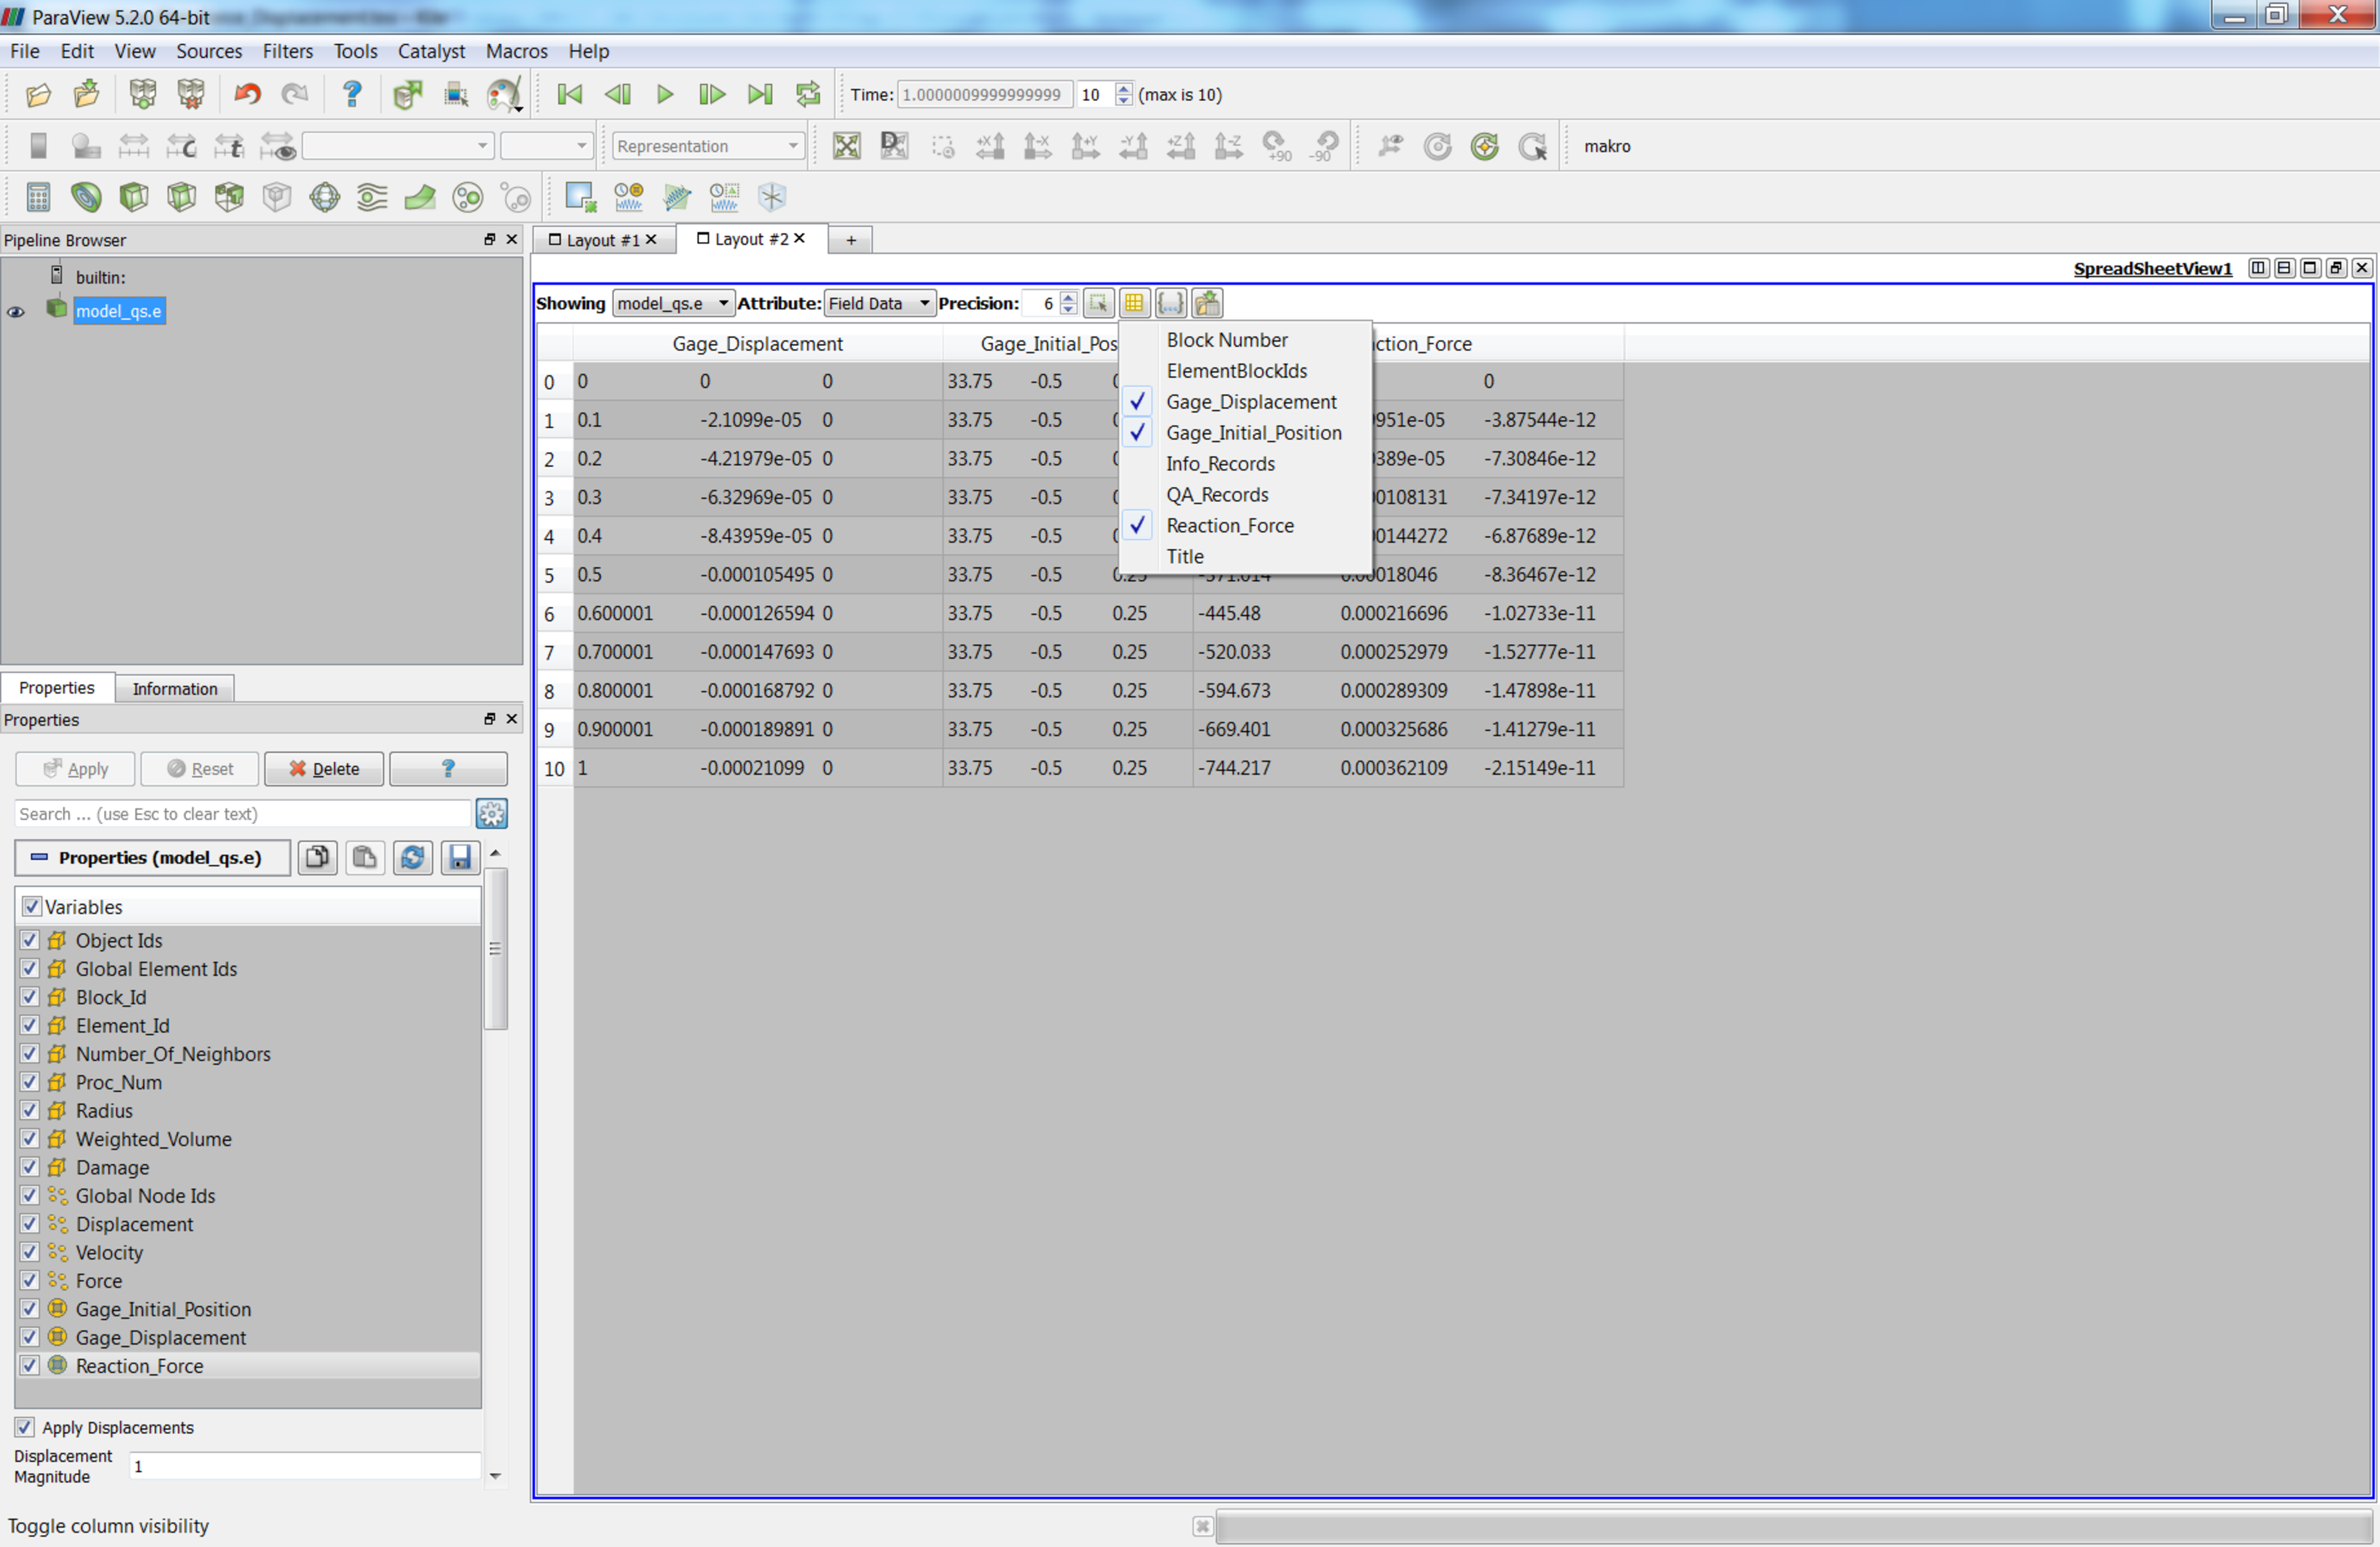
\includegraphics[width=\linewidth]{Figures/Screenshots/ParaView_ComputeClassParameter_ResultsData_2}};
      \begin{scope}[
        x={(image.south east)},
        y={(image.north west)},
      ]
        % Some label
        \node[fit={(0.22,0.785) (0.40,0.82)},myrectangularmarkup] (rect3) {};
        \node[anchor=north,mymarkuptext] (rect3label) at (rect3.south) {3};
        %
        \node[fit={(0.465,0.62) (0.585,0.82)},myrectangularmarkup] (rect4) {};
        \node[anchor=west,mymarkuptext] (rect4label) at (rect4.east) {4};
        % Help grid and labels
        %\pic{myimagegrid};
      \end{scope}
      % Outside label
    \end{tikzpicture}
    \caption{Steps 3-4}
    \label{fig:ParaView_ComputeClassParameter_ResultsData_2}
  \end{subfigure}%
\caption{Access \texttt{Compute Class Parameters} results data in \protect\paraviewname}
\label{fig:Use_ParaView_ComputeClassParameter_ResultsData}
\end{figure}

\begin{enumerate}[noitemsep]
  \item Make sure that the requested result data from the \textit{Compute Class Parameters} is available in your results file. If you are only interested in these parameters, unselect all other.
  \item Add a new view \& select \textit{SpreadSheet View}
  \item For \textit{Showing} select your model and for \textit{Attribute} select \textit{Field Data}
  \item Click 
\includegraphics[width=\iconsize]{Figures/Icons/pqRectilinearGrid16} to select the columns of interest
  \item Click 
\includegraphics[width=\iconsize]{Figures/Icons/pqSaveTable32} to save the spreadsheet data as a \texttt{csv}-file
  \begin{enumerate}[noitemsep]
    \item Specify a filename \& click \textit{Ok}
    \item In the next dialog toggle \textit{Filter Columns by Visibility}. Otherwise, all data is written to the \texttt{csv}-file.
  \end{enumerate}
  \item Do with the data whatever you want \smiley
\end{enumerate}

\levelstay{Plot result data directly in \protect\paraviewname}

\begin{figure}[htbp]
\centering
    \begin{tikzpicture}
      % External figure
      \node[anchor=south west,inner sep=0] (image) at (0,0) {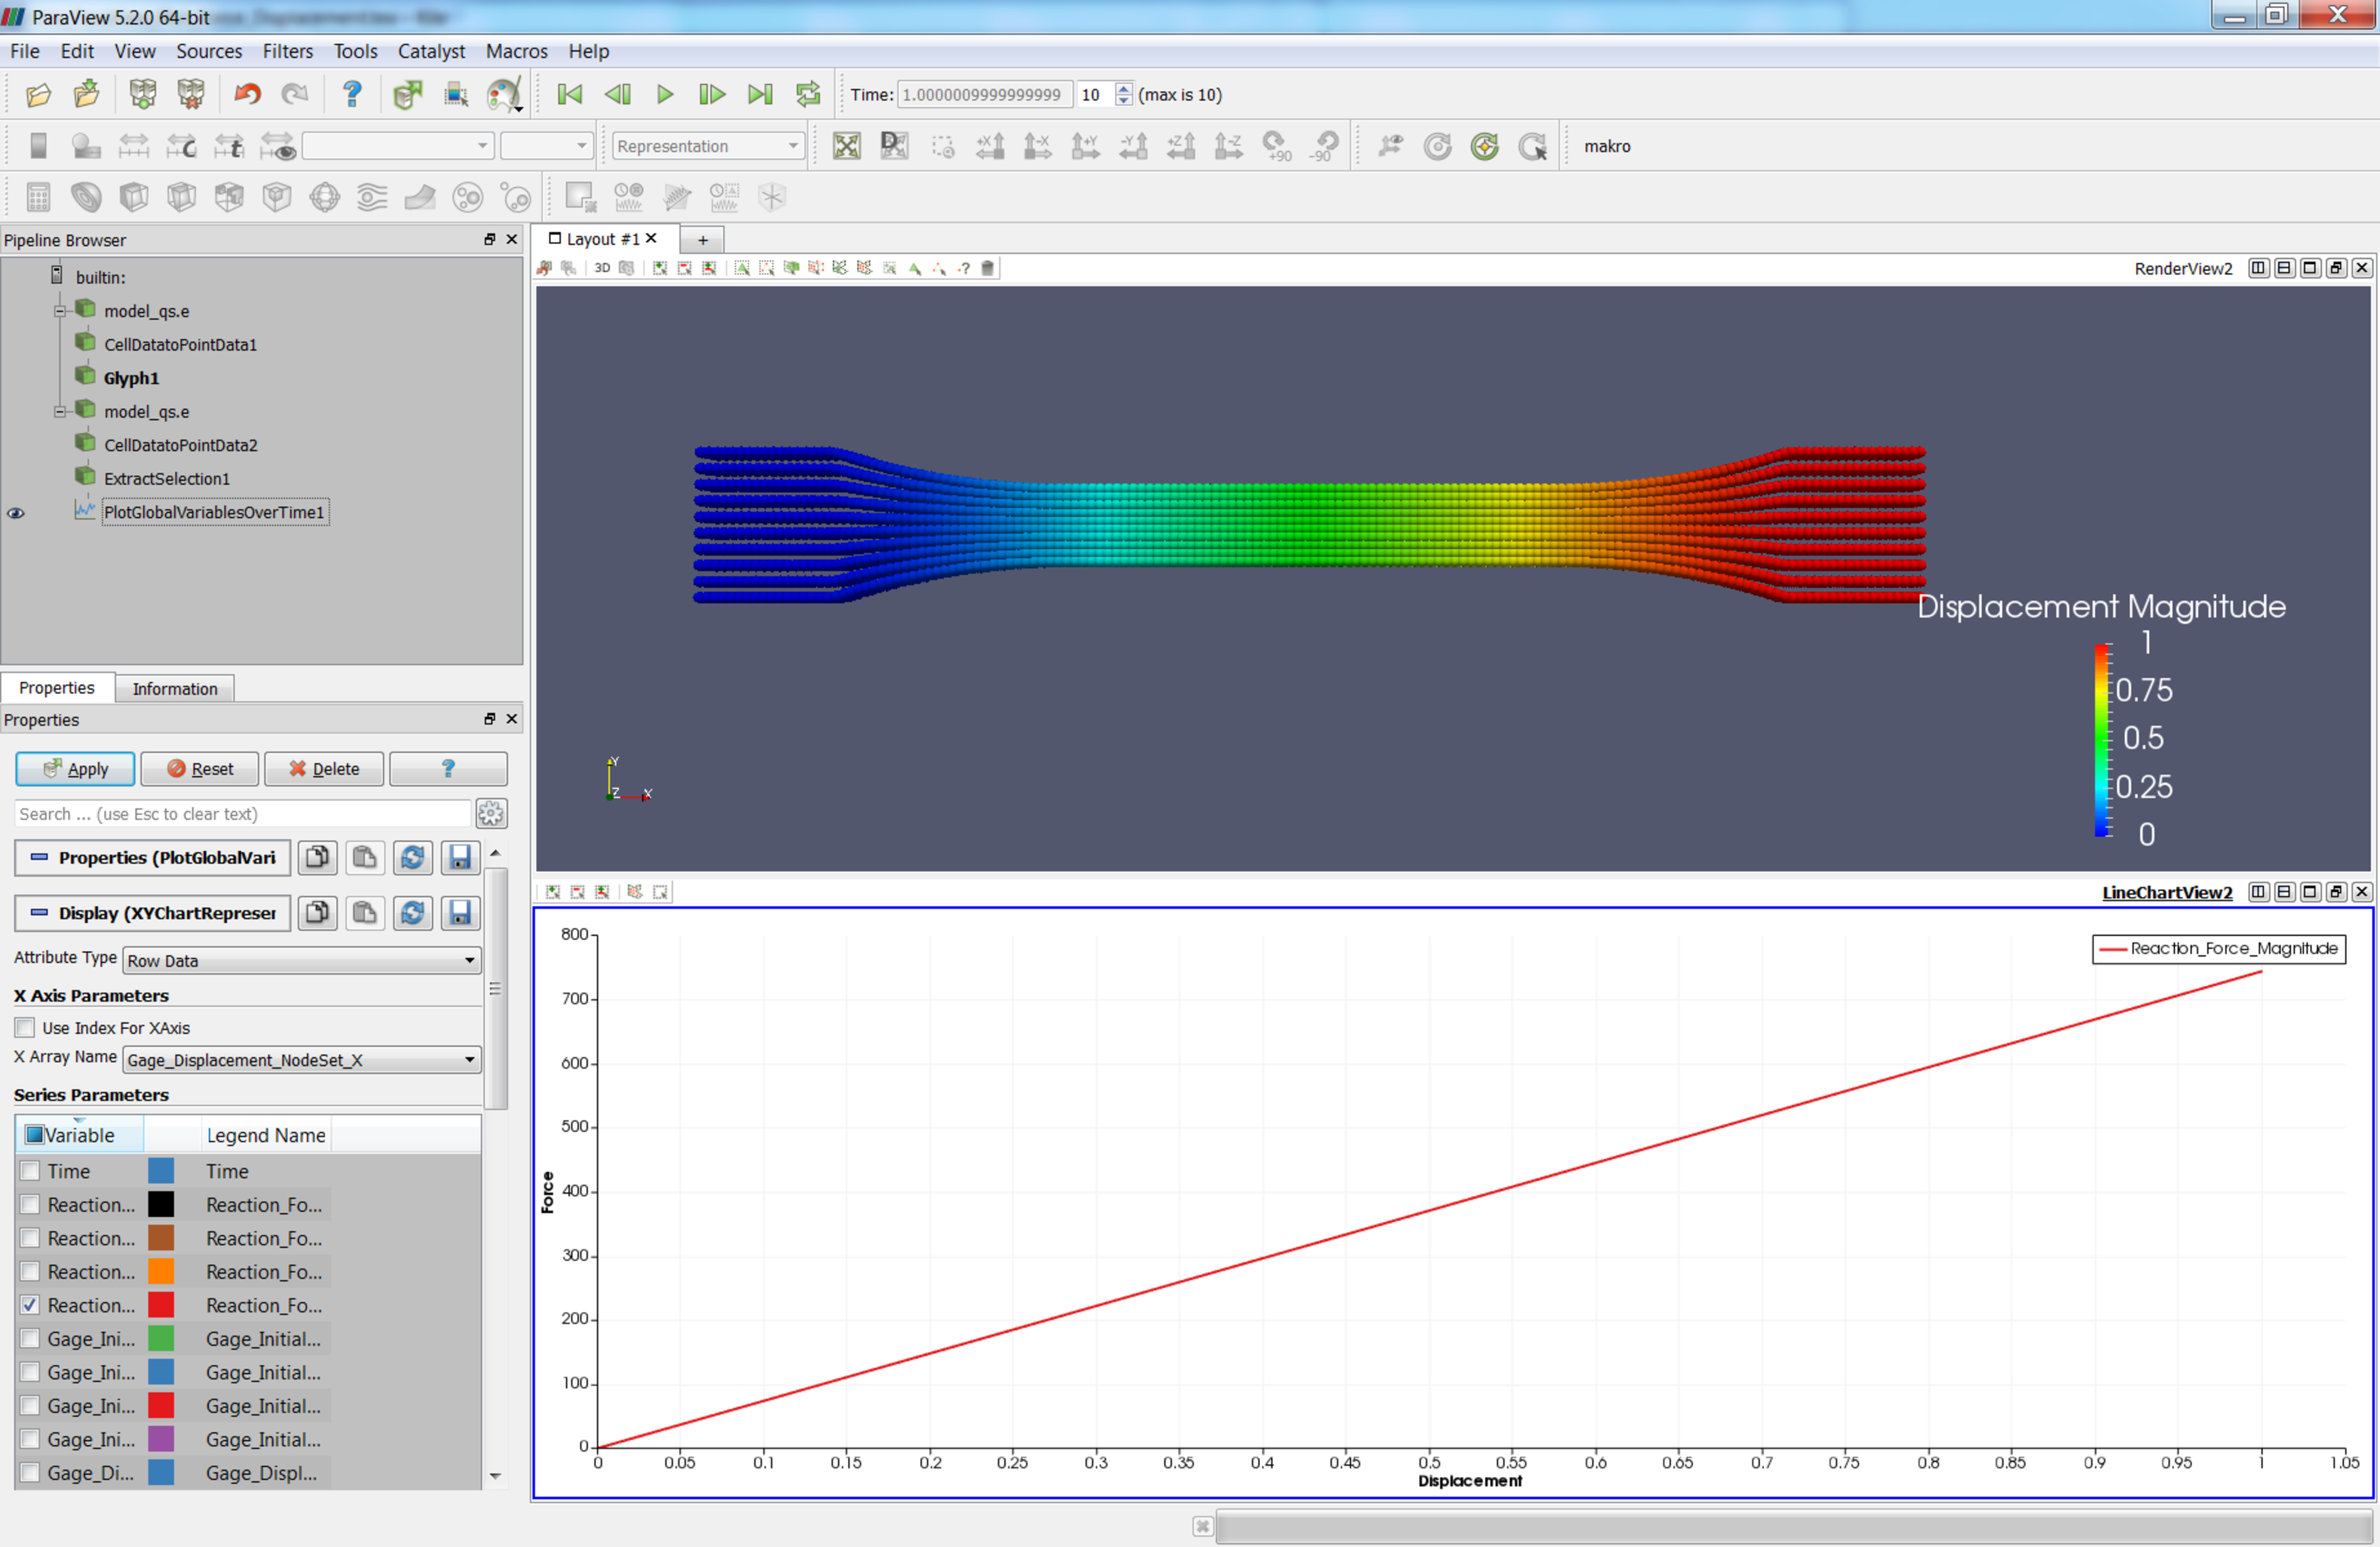
\includegraphics[width=0.8\linewidth]{Figures/Screenshots/ParaView_ComputeClassParameter_ResultsData_3}};
      \begin{scope}[
        x={(image.south east)},
        y={(image.north west)},
      ]
        % Some label
%         \node[fit={(0.007,0.10) (0.18,0.17)},myrectangularmarkup] (rect1) {};
%         \node[anchor=west,mymarkuptext] (rect1label) at (rect1.east) {1};
%         %
%         \node[fit={(0.280,0.83) (0.31,0.86)},myrectangularmarkup] (rect2) {};
%         \node[anchor=west,mymarkuptext] (rect2label) at (rect2.east) {2};
        % Help grid and labels
%         \pic{myimagegrid};
      \end{scope}
    \end{tikzpicture}
\caption{Plot \texttt{Compute Class Parameters} results data in \protect\paraviewname}
\label{fig:Use_ParaView_ComputeClassParameter_ResultsData_ForceDisplacement_in-ParaView}
\end{figure}

\begin{enumerate}[noitemsep]
  \item Import your model
  \item Make sure that the requested result data from the \textit{Compute Class Parameters} is available in your results file. If you are only interested in these parameters, unselect all other.
  \item From the menu bar:
    \begin{itemize}[noitemsep]
    \item Click Filters
    \item Click Alphabetical
    \item Click \textit{Cell Data to Point Data}
    \end{itemize}
  \item Select points of interest:
    \begin{itemize}[noitemsep]
    \item Select the \textit{Cell Data to Point Data} entry in the Pipeline Browser
    \item Create a new selection of a single or multiple points in your constraint region as described in \autoref{sec:Use_ParaView_Selection_Create}
    \item Extract the selection as described in \autoref{sec:Use_ParaView_Selection_LimitTo}
    \end{itemize}
  \item From the menu bar:
    \begin{itemize}[noitemsep]
    \item Click Filters
    \item Click Data Analysis
    \item Click \textit{Plot Selection Over Time}
    \end{itemize}
    or click 
\includegraphics[width=\iconsize]{Figures/Icons/pqPlotSelectionOverTime24} in the Data Analysis toolbar
  \item Preferences in the \textit{Properties} window
    \begin{itemize}[noitemsep]
    \item Under \textit{X Axis Parameters} select your displacement component or magnitude from the \texttt{Compute Class Parameters} in the \textit{X Array Name} combobox
    \item For \textit{Series Parameters} select the force value you want to plot from the \texttt{Compute Class Parameters}, either as a component or magnitude
    \item Input a \textit{Left Axis Title} and \textit{Bottom Axis Title} if required
    \end{itemize}
  \item Click \textit{Apply}
  \item In case you want to export the chart data from here:
    \begin{itemize}[noitemsep]
    \item Left-click on the chart
    \item From the menu bar:
      \begin{itemize}[noitemsep]
      \item Click \textit{File}
      \item Click \textit{Save As}
      \item Export as \texttt{csv}-file
      \end{itemize}
    \end{itemize}
\end{enumerate}

\levelup{\protect\abaqusname}

% https://www.youtube.com/watch?v=O8CcSB11468

\leveldown{Standard}

\begin{enumerate}[noitemsep]
  \item Choose Displacement (U) \& Reaction Forces (RF) as field outputs for the step you want to have the plot
  \item Run the analysis
  \item Open the odb
  \item Reaction force over time:
  \begin{enumerate}[noitemsep]
    \item Click \textit{Create XY Data}
    \item Select Source \textit{ODB history output}
    \item Click \textit{Continue}
    \item Select all entries with beginning \textit{Reation force:} of the nodeset your are interested in
    \item Click \textit{Save as}
    \item Assign name, here ``RF'', \& in \textit{Save Operation} select \textit{sum((XY,XY,$\ldots$))}
  \end{enumerate}
  \item Displacement over time:
  \begin{enumerate}[noitemsep]
    \item Click \textit{Create XY Data}
    \item Select Source \textit{ODB history output}
    \item Click \textit{Continue}
    \item Select all entries with beginning \textit{Spatial displacement Ui:} of the nodeset your are interested in
    \item Click \textit{Save as}
    \item Assign name, here ``U'', \& in \textit{Save Operation} select \textit{avg((XY,XY,$\ldots$))}
  \end{enumerate}
  \item Reaction force over displacement:
  \begin{enumerate}[noitemsep]
    \item Click \textit{Create XY Data}
    \item Select Source \textit{Operate on XY data}
    \item Click \textit{Continue}
    \item From \textit{Operators} select \textit{Combine}
    \item In the equation, at first select ``U'', than ``RF'', the equation than should be \verb+combine ("U","F")+
    \item Select \textit{Plot Expression}
  \end{enumerate}
\end{enumerate}

\levelstay{Explicit}

\begin{enumerate}[noitemsep]
  \item Choose Displacement (U), Reaction Forces (RF) \& Nodal forces (NFORC) as field outputs for the step you want to have the plot
  \item Run the analysis
  \item Open the odb
  \item Reaction force \& Displacement over time:
  \begin{enumerate}[noitemsep]
    \item Click \textit{Create XY Data}
    \item Select Source \textit{ODB field output}
    \item Click \textit{Continue}
    \item \textit{XY Data from ODB Field Output} dialog:
      \begin{enumerate}[noitemsep]
        \item In the \textit{Variables} tab, select \textit{Unique nodal} in the \textit{Position} combobox and all necessary entry checkboxes, here RF1 and U1
        \item In the \textit{Elements/Nodes} tab, select the requested nodeset
      \end{enumerate}
    \item Click \textit{Save}
  \end{enumerate}
  \item Sum forces:
  \begin{enumerate}[noitemsep]
    \item Click \textit{Create XY Data}
    \item Select Source \textit{Operate on XY data}
    \item From \textit{Operators} select \textit{sum}
    \item In the equation, select all ``RF1'' entries`` and click \textit{Add to expression}
    \item Click \textit{Save as} \& assign name ''RF``
  \end{enumerate}
  \item Average displacements:
  \begin{enumerate}[noitemsep]
    \item Click \textit{Create XY Data}
    \item Select Source \textit{Operate on XY data}
    \item From \textit{Operators} select \textit{avg}
    \item In the equation, select all ``U1'' entries`` and click \textit{Add to expression}
    \item Click \textit{Save as} \& assign name ''U``
  \end{enumerate}
  \item Reaction force over displacement:
  \begin{enumerate}[noitemsep]
    \item Click \textit{Create XY Data}
    \item Select Source \textit{Operate on XY data}
    \item Click \textit{Continue}
    \item From \textit{Operators} select \textit{Combine}
    \item In the equation, at first select ``U'', than ``RF'', the equation than should be \verb+combine ("U","F")+
    \item Select \textit{Plot Expression}
  \end{enumerate}
\end{enumerate}

\levelstay{Save XY data}

\begin{enumerate}[noitemsep]
  \item Open the odb
  \item Create all results
  \item In the menu bar, click \textit{Report}
  \item Click \textit{XY}
  \item Adjust the dialog preferences according to your needs
\end{enumerate}

\newpage
%%%%%%%%%%%%%%%%%%%%%%%%%%%%%%%%%%%%
% Header                           %
%%%%%%%%%%%%%%%%%%%%%%%%%%%%%%%%%%%%
% 
% Revisions: 2017-04-10 Martin R�del <martin.raedel@dlr.de>
%                       Initial draft
%               
% Contact:   Martin R�del,  martin.raedel@dlr.de
%            DLR Composite Structures and Adaptive Systems
%          
%                                 __/|__
%                                /_/_/_/  
%            www.dlr.de/fa/en      |/ DLR
% 
%%%%%%%%%%%%%%%%%%%%%%%%%%%%%%%%%%%%
% Content                          %
%%%%%%%%%%%%%%%%%%%%%%%%%%%%%%%%%%%%

\levelmultiup{Measuring}{3}

%%%%%%%%%%%%%%%%%%%%%%%%%%%%%%%%%%%%
% Header                           %
%%%%%%%%%%%%%%%%%%%%%%%%%%%%%%%%%%%%
% 
% Revisions: 2017-04-10 Martin R�del <martin.raedel@dlr.de>
%                       Initial draft
%               
% Contact:   Martin R�del,  martin.raedel@dlr.de
%            DLR Composite Structures and Adaptive Systems
%          
%                                 __/|__
%                                /_/_/_/  
%            www.dlr.de/fa/en      |/ DLR
% 
%%%%%%%%%%%%%%%%%%%%%%%%%%%%%%%%%%%%
% Content                          %
%%%%%%%%%%%%%%%%%%%%%%%%%%%%%%%%%%%%

\leveldown{Node/point position}

Sometimes it is necessary to get the exact position of a single point or selection of points. The following steps give you these informations and are explained for a selection of points. For an inidividual point some steps can be omitted.

\begin{enumerate}[noitemsep]
  \item Import the model
  \item Generate and extract the selection of interest according to \autoref{sec:Use_ParaView_Selection}
  \item Display the node/point numbers according to \autoref{sec:Paraview:Display:Point:Labels}
  \item Remember the node/point numbers
  \item In the RenderView select \textit{Split Horizontal}
  \item Create a new SpreadSheet View
  \item In the SpreadSheet View:
  \begin{itemize}[noitemsep]
    \item Select your selection in the \textit{Showing} combobox
    \item Select \textit{Point Data} in the \textit{Attribute} combobox
    \item The coordinates appear in the \textit{Points} column of the table
    \item In case not all your selected points appear in the table, check if the blocks the points are part of are selected in the \textit{Properties tab} of your selection
  \end{itemize}
  \item Unfortunately the node/point number labels disappear
\end{enumerate}

\begin{figure}[htbp]
\centering
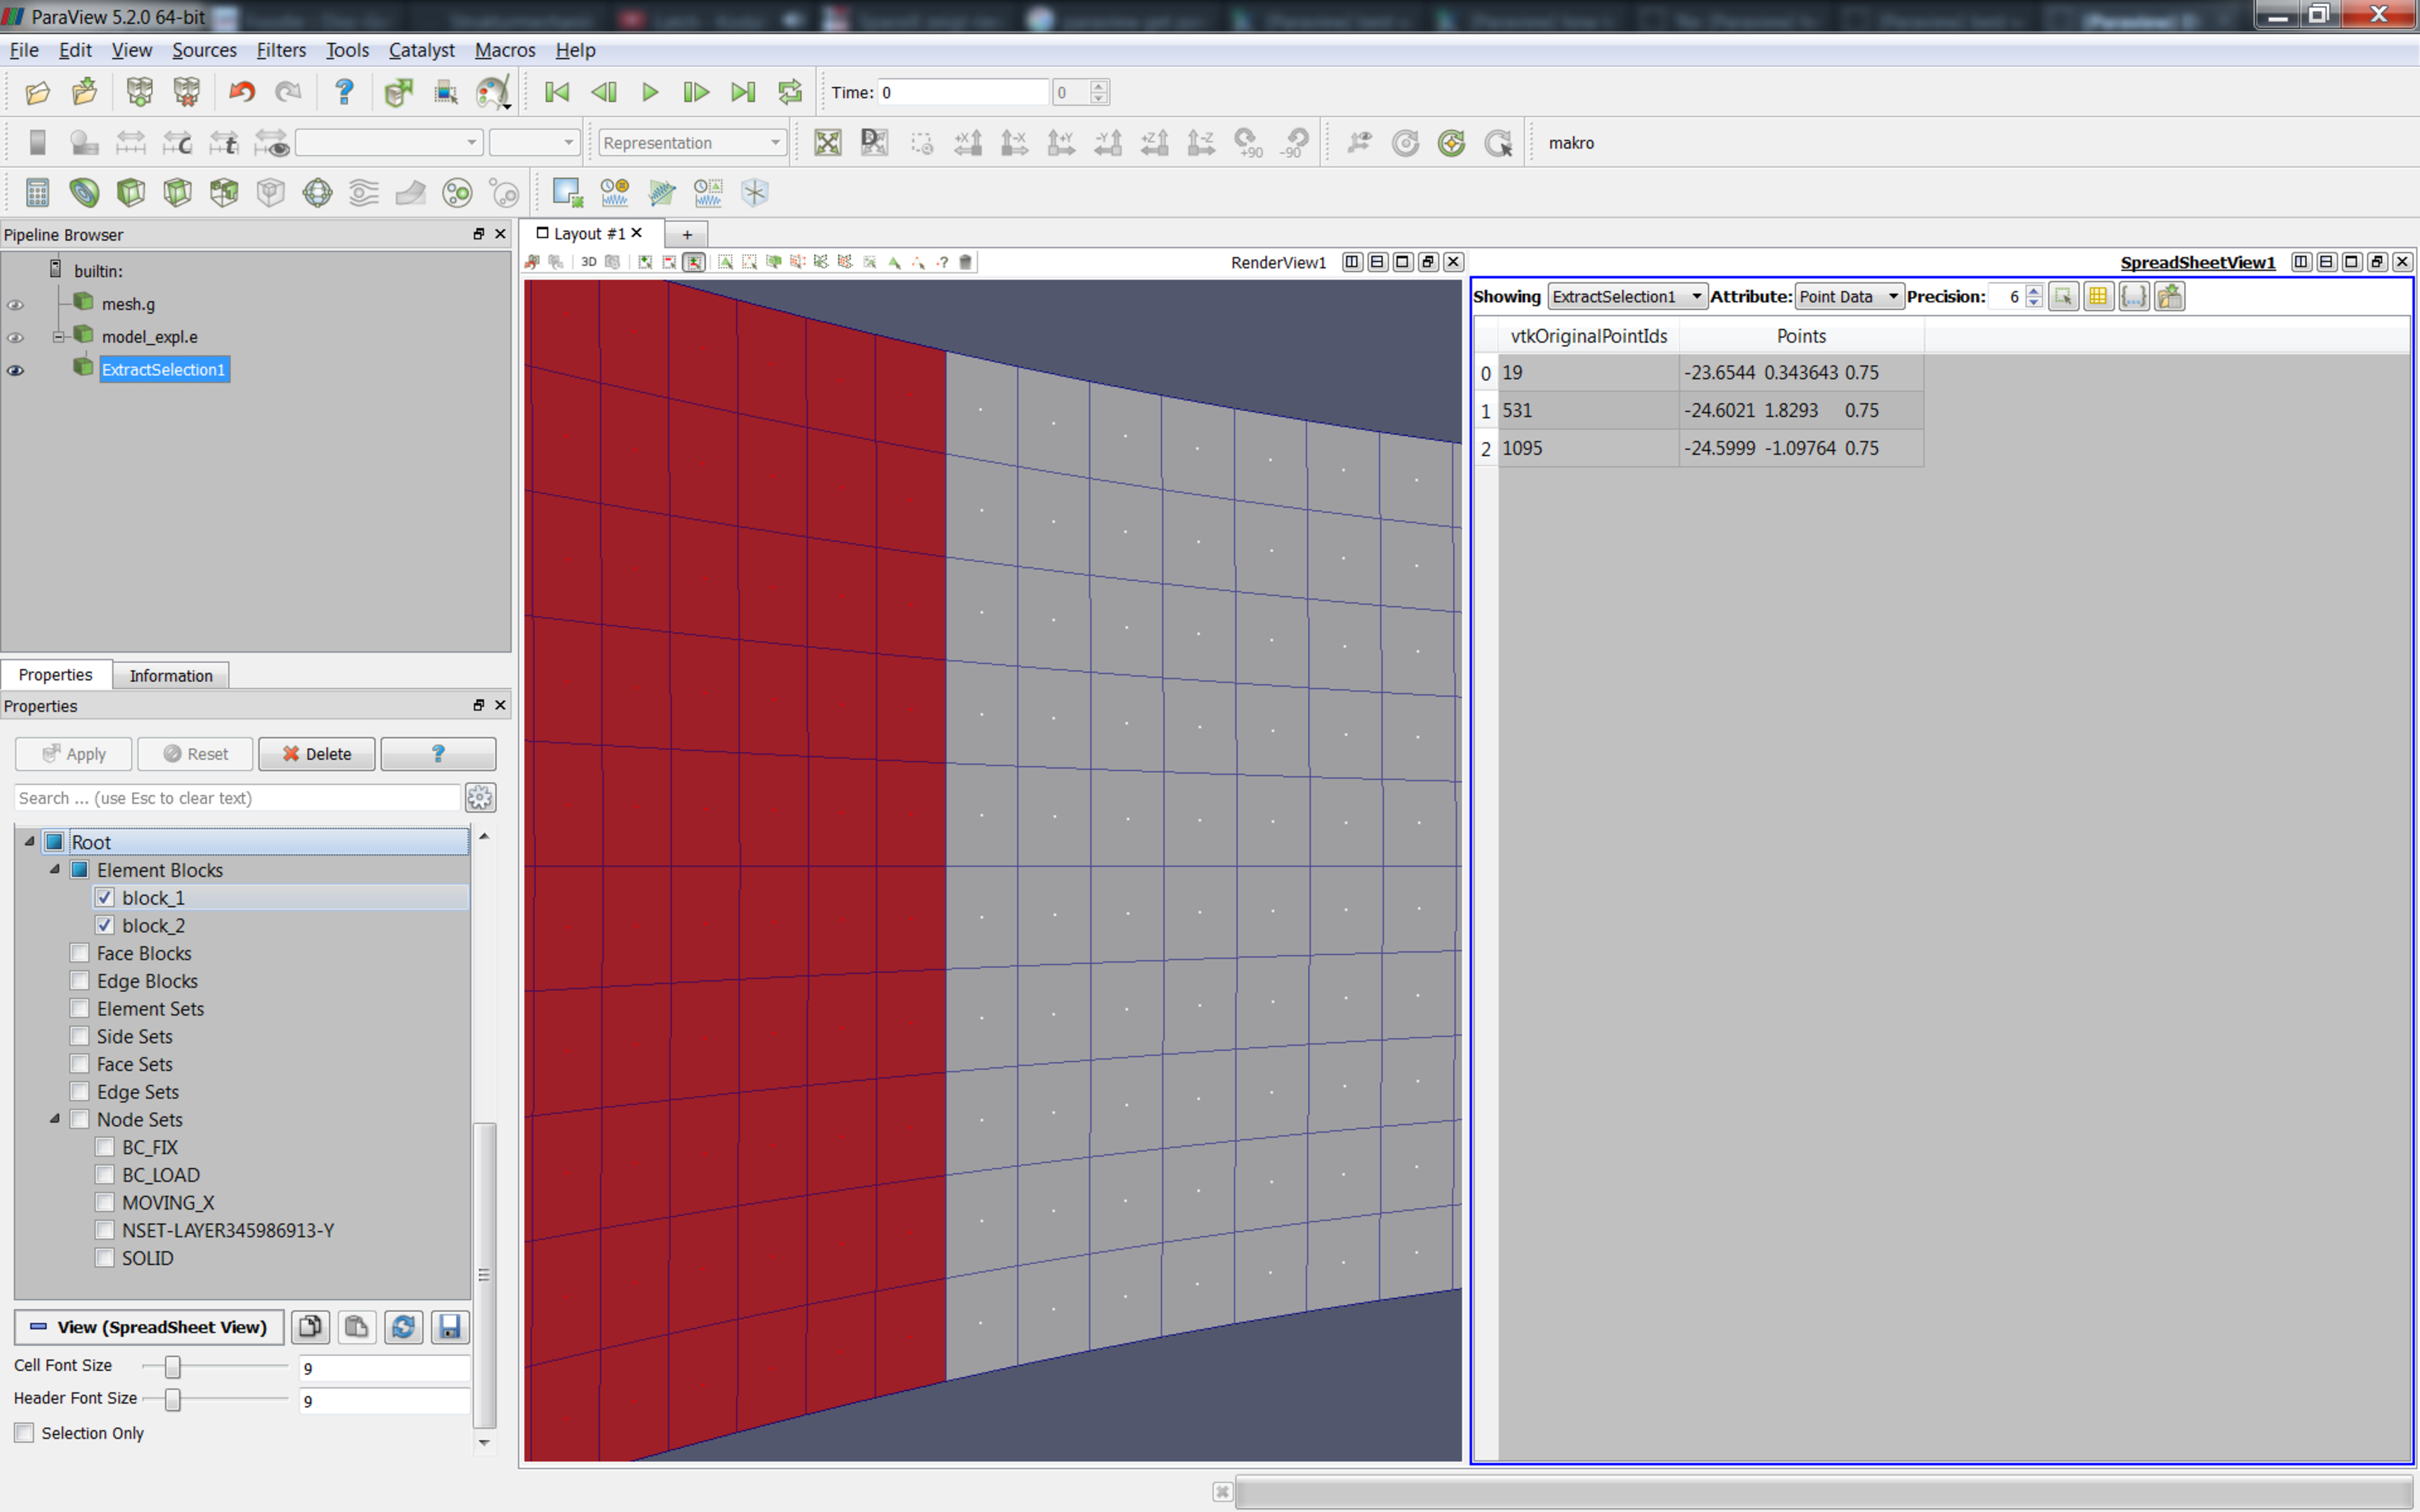
\includegraphics[width=\paraviewscreenshotwidthfac\linewidth]{Figures/Screenshots/ParaView_Display_NodePosition}
\caption{Display of selection point/node positions}
\label{fig:Use_ParaView_Display_NodePositions}
\end{figure}

%%%%%%%%%%%%%%%%%%%%%%%%%%%%%%%%%%%%
% Header                           %
%%%%%%%%%%%%%%%%%%%%%%%%%%%%%%%%%%%%
% 
% Revisions: 2017-04-10 Martin R�del <martin.raedel@dlr.de>
%                       Initial draft
%               
% Contact:   Martin R�del,  martin.raedel@dlr.de
%            DLR Composite Structures and Adaptive Systems
%          
%                                 __/|__
%                                /_/_/_/  
%            www.dlr.de/fa/en      |/ DLR
% 
%%%%%%%%%%%%%%%%%%%%%%%%%%%%%%%%%%%%
% Content                          %
%%%%%%%%%%%%%%%%%%%%%%%%%%%%%%%%%%%%

\levelstay{Node/point distance}

\begin{figure}[htbp]
\centering
  \begin{tikzpicture}
    % External figure
    \node[anchor=south west,inner sep=0] (image) at (0,0) {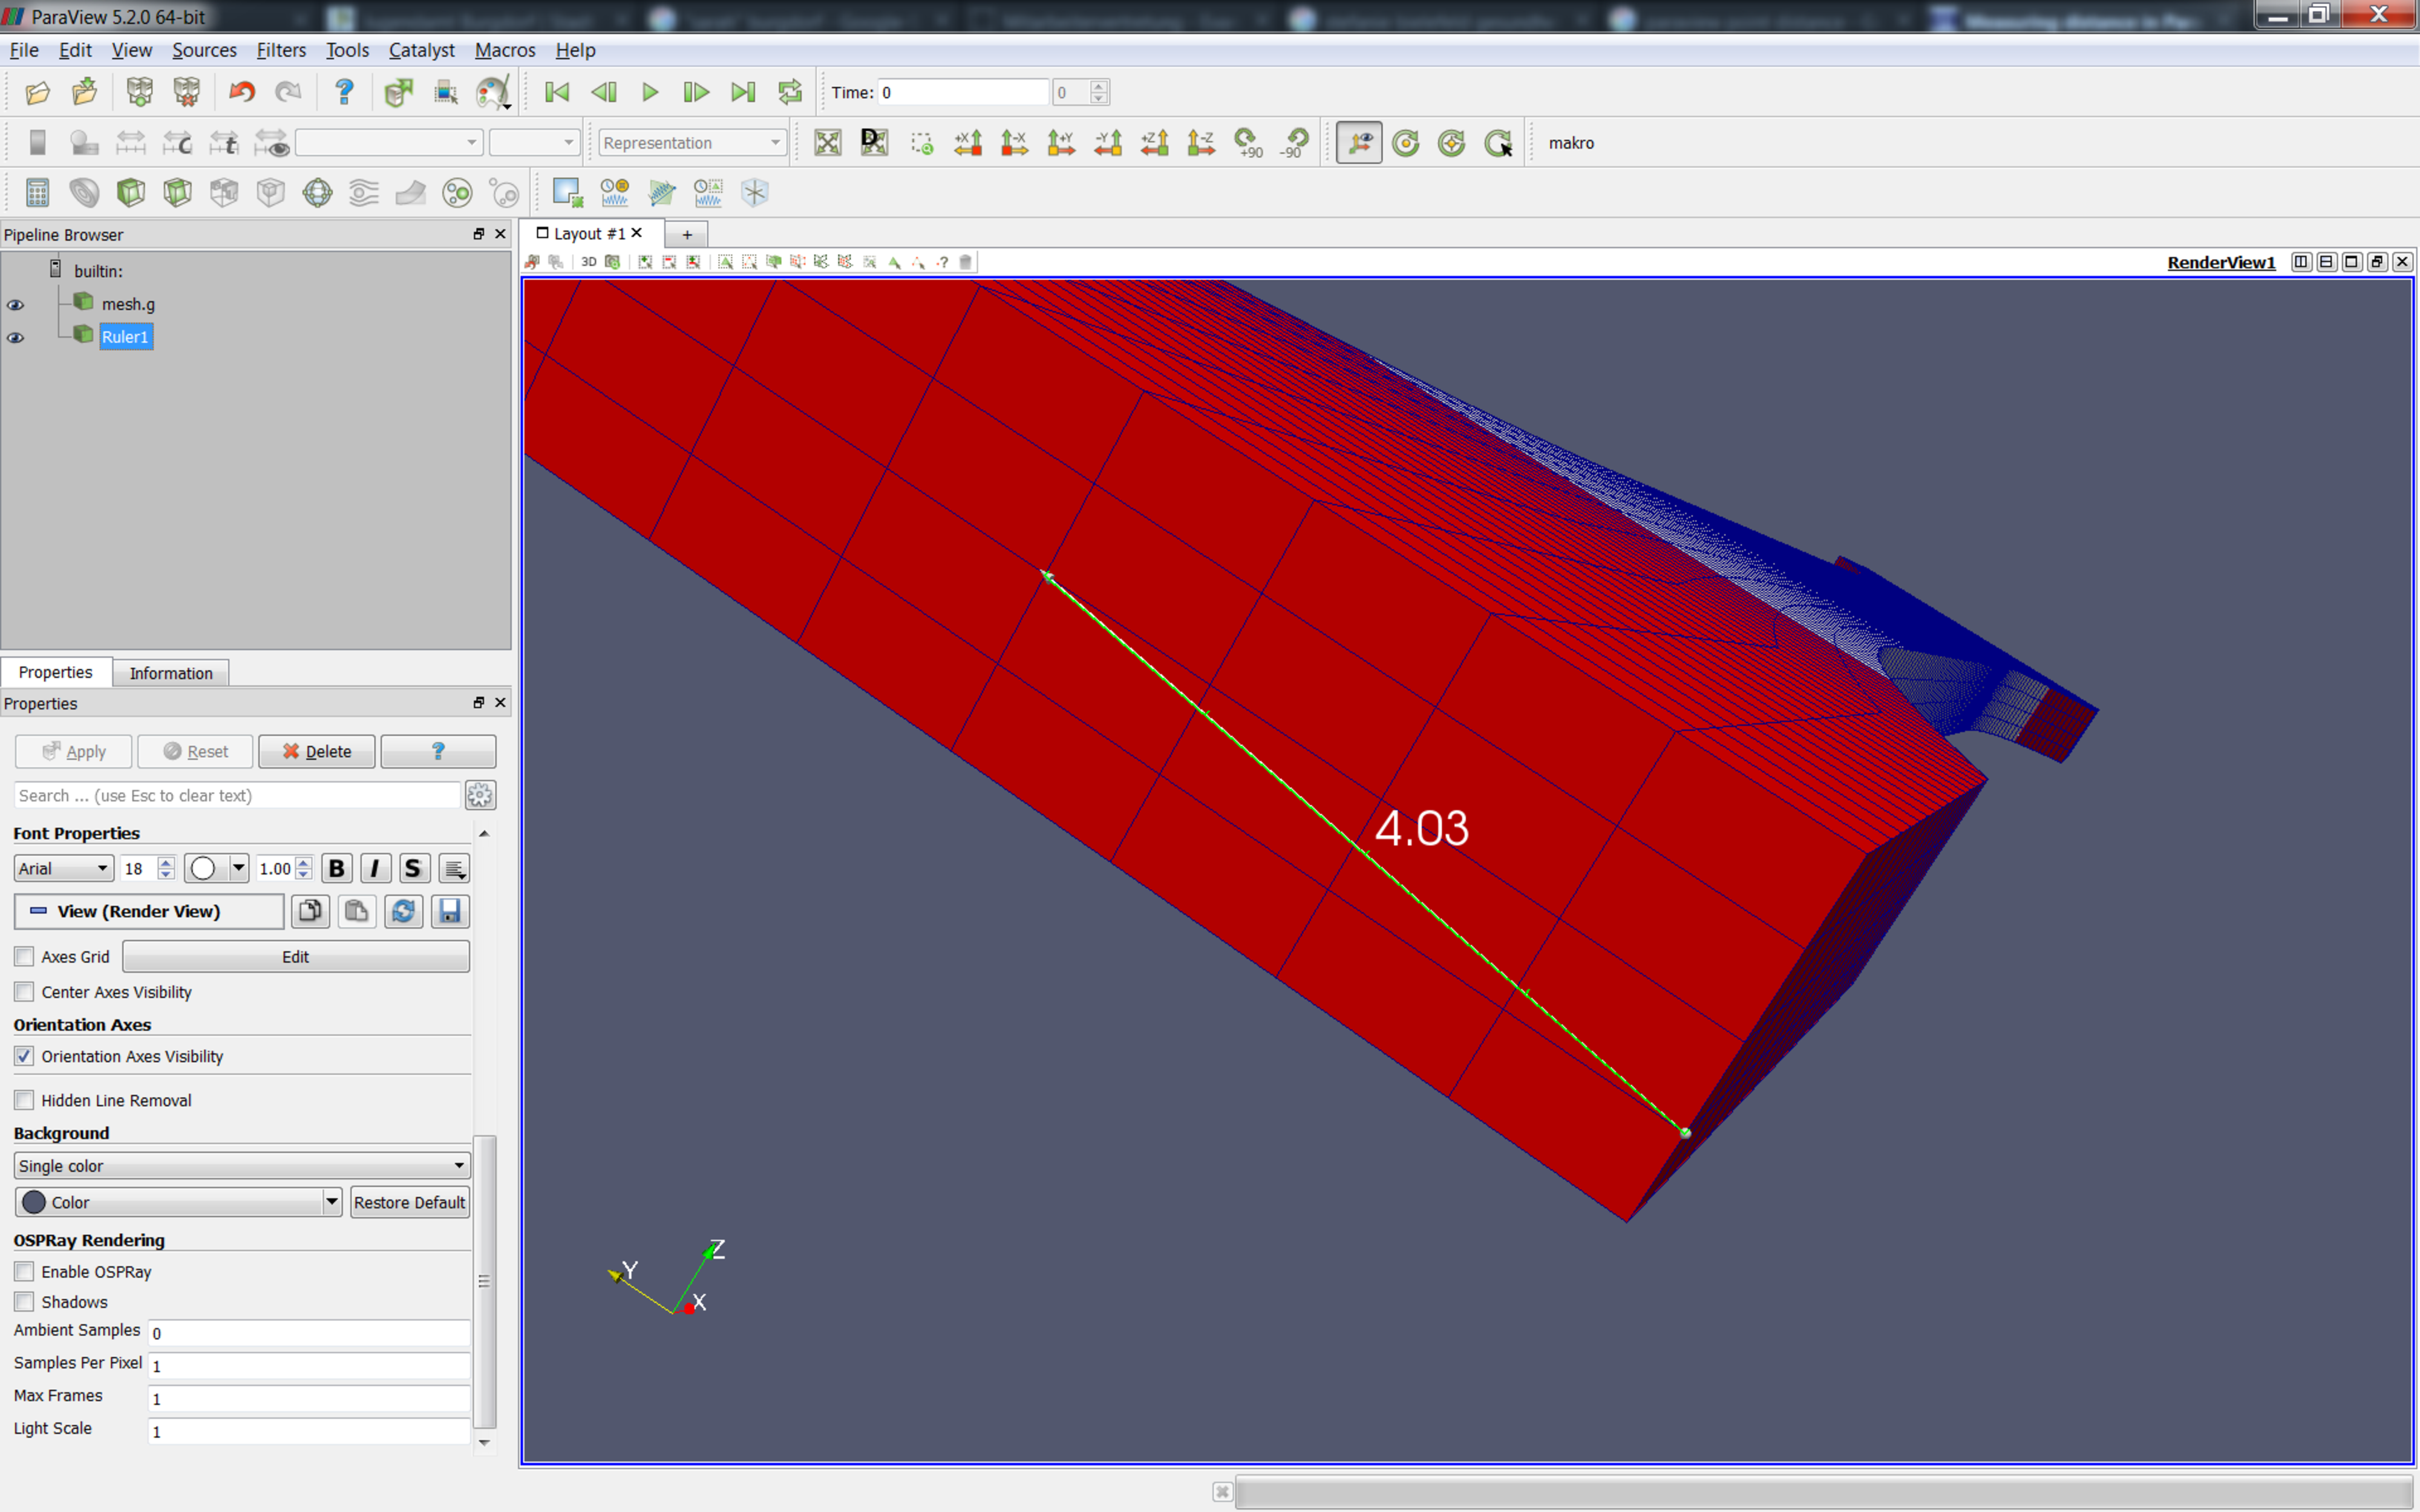
\includegraphics[width=\paraviewscreenshotwidthfac\linewidth]{Figures/Screenshots/ParaView_Measure_NodeDistance}};
    \begin{scope}[
      x={(image.south east)},
      y={(image.north west)},
    ]
      % Some label
%         \node[fit={(0.007,0.10) (0.18,0.17)},myrectangularmarkup] (rect1) {};
%         \node[anchor=west,mymarkuptext] (rect1label) at (rect1.east) {1};
%         %
%         \node[fit={(0.280,0.83) (0.31,0.86)},myrectangularmarkup] (rect2) {};
%         \node[anchor=west,mymarkuptext] (rect2label) at (rect2.east) {2};
      % Help grid and labels
%       \pic{myimagegrid};
    \end{scope}
  \end{tikzpicture}
\caption{Measure point distance in \protect\paraviewname}
\label{fig:Use_ParaView_Measure_NodeDistance}
\end{figure}

To measure the distance between two nodes or collocation points after importing the model:

\begin{enumerate}[noitemsep]
  \item In the menu bar
  \begin{itemize}[noitemsep]
    \item Click on \textit{Sources}
    \item Click \textit{Ruler}
  \end{itemize}
  \item In the render view
  \begin{itemize}[noitemsep]
    \item Left-click the first point and keep the mouse clicked
    \item Move the point close to the target
    \item Press ``CTRL+1'' and snap the point to the closest mesh point
    \item Do the same for the second point, but press ``CTRL+2'' instead for snapping
  \end{itemize}
  \item In the \textit{Ruler} properties window
  \begin{itemize}[noitemsep]
    \item Adjust preferences to your need
    \item Click \textit{Apply}
  \end{itemize}
  \item The number next to the \textit{Ruler} in the render view is the point distance
\end{enumerate}


\newpage
%%%%%%%%%%%%%%%%%%%%%%%%%%%%%%%%%%%%
% Header                           %
%%%%%%%%%%%%%%%%%%%%%%%%%%%%%%%%%%%%
% 
% Revisions: 2017-04-10 Martin R�del <martin.raedel@dlr.de>
%                       Initial draft
%               
% Contact:   Martin R�del,  martin.raedel@dlr.de
%            DLR Composite Structures and Adaptive Systems
%          
%                                 __/|__
%                                /_/_/_/  
%            www.dlr.de/fa/en      |/ DLR
% 
%%%%%%%%%%%%%%%%%%%%%%%%%%%%%%%%%%%%
% Content                          %
%%%%%%%%%%%%%%%%%%%%%%%%%%%%%%%%%%%%

\levelup{Exporting}
\leveldown{Quick Screenshot}

Screenshot are taken from the current view you see in \marktool{\paraviewname} render view. Therefore, perform all adjustments to the view to your needs before creating a screenshot.

To save a screenshot from \marktool{\paraviewname} perform the following steps:

\begin{enumerate}[noitemsep]
\item Click \textit{File} in the menubar
\item Click \textit{Save Screenshot}
\item Set plot preferences:
  \begin{itemize}[noitemsep]
  \item Uncheck \textit{Save only selected view} if necessary
  \item Activate the \textit{Lock aspect} button right of the resolution
  \item Change the resolution to values high enough for a print-quality picture\\(the higher value should at least be 1000)
  \item \textit{Select image quality} slider \tab 100
  \item Override color palette:	\tab \textit{Current palette}
  \item Stereo Mode:		\tab \textit{No stereo}
  \end{itemize}
\item Click \textit{Ok}
\item Specify the path and \textit{File name}
\item Choose \textit{PNG image} as file type
\item Click \textit{Ok}
\end{enumerate}

Afterwards, use \marktool{GIMP}, \marktool{Inkscape}, \marktool{convert} utility from \marktool{ImageMagick} or any other tool to convert the pixel to a non-scalable vector graphics copy as \verb+eps+ and \verb+pdf+ copy.

For the sake of reproducibility of the created picture save the \marktool{\paraviewname} state as described in section \ref{sec:Paraview_Save_States}.

The target must be to have the figure and the \marktool{\paraviewname} state file available at all time:

\begin{code}
figure_name.eps
figure_name.pdf
figure_name.png
figure_name.pvsm
\end{code}

\levelstay{Vector graphics - kind of}

The vector graphics output only affects the non-3D rendered elements such as texts, cube axes etc. Normal or glyph plots which are 3D rendered are not affected. Therefore, this option is currently no use for the documentation. It is proposed to create high-quality png-plot with the \textit{Save Screenshot} function and use \marktool{GIMP}, \marktool{Inkscape}, \marktool{convert} utility from \marktool{ImageMagick} or any other tool to convert the pixel to a non-scalable vector graphics copy.

\levelstay{Animations}	\label{sec:ParaView_Save_Animation}

\marktool{\paraviewname} allows the creation of animations for your currently selected view entity. So choose your plot coloring and vector entities before creating an animation.

To save an animation from \marktool{\paraviewname} perform the following steps:

\begin{enumerate}[noitemsep]
\item Click \textit{File} in the menubar
\item Click \textit{Save Animation}
\item Set animation preferences:
  \begin{itemize}[noitemsep]
  \item Animation duration:	\tab -
  \item Frame rate:		\tab $\ge$15	\\
  The human brain perceives successive images as moving, but not necessarily smooth, scene from about 14 to 16 frames per second.
  \item No. of Frames/timestep:	\tab 1
  \item Number of Frames:	\tab -
  \item Resolution:		\tab higher value $\ge$ 1000
  \item Timestep Range:		\tab Start- and end time step of interest
  \item Stereo Mode:		\tab \textit{No Stereo}
  \item Compression:		\tab Checked
  \end{itemize}
\item Click \textit{Save Animation}
\item Specify the path and \textit{File name}
\item Choose the file type of your liking, either video or multiple images
\item Click \textit{Ok}
\end{enumerate}

For the sake of reproducibility of the created animation save the \marktool{\paraviewname} state as described in section \ref{sec:Paraview_Save_States}.

The target must be to have the animation and the \marktool{\paraviewname} state file available at all time:

\begin{code}
animation_name.avi
animation_name.pvsm
\end{code}

\levelstay{Save \texorpdfstring{\protect\marktool{\paraviewname}}{\paraviewname{}} states for exported items}	\label{sec:Paraview_Save_States}

For the sake of reproducibility of the created picture or animation you can save the \marktool{\paraviewname} state. If you want to reproduce the picture or animation you can just load the state and all preferences will be set to the exact values of the saved state.

To save a state perform the following steps:

\begin{enumerate}[noitemsep]
\item Click \textit{File} in the menubar
\item Click \textit{Save State}
\item Specify the path of the figure or animation directory and the \textit{File name} identical to the figure file name
\item Choose \textit{ParaView state file (*.pvsm)} as file type
\item Click \textit{Ok}
\end{enumerate}

A state can be loaded accordingly:

\begin{enumerate}[noitemsep]
\item Click \textit{File} in the menubar
\item Click \textit{Load State}
\item Select the state file
\item Click \textit{Ok}
\end{enumerate}

\newpage
%%%%%%%%%%%%%%%%%%%%%%%%%%%%%%%%%%%%
% Header                           %
%%%%%%%%%%%%%%%%%%%%%%%%%%%%%%%%%%%%
% 
% Revisions: 2017-04-10 Martin R�del <martin.raedel@dlr.de>
%                       Initial draft
%               
% Contact:   Martin R�del,  martin.raedel@dlr.de
%            DLR Composite Structures and Adaptive Systems
%          
%                                 __/|__
%                                /_/_/_/  
%            www.dlr.de/fa/en      |/ DLR
% 
%%%%%%%%%%%%%%%%%%%%%%%%%%%%%%%%%%%%
% Content                          %
%%%%%%%%%%%%%%%%%%%%%%%%%%%%%%%%%%%%

\levelup{Preferences}

\leveldown{Change mesh on sphere \texttt{Glyph}}

Sometimes for nice publication pictures the default sphere glyph representation might be a little too angular. Internally, sphere glyphs are nothing but a combination of a certain number of tetrahedron elements. Thus, the mesh behind a sphere glyph might be too coarse. It is assumed you already have a glyph as spheres, otherwise have a look at \autoref{sec:ParaView_Damage_Plots_on_Nodes_as_Spheres}. 

In order to change the mesh size and smooth the sphere shape perform the following steps:

\begin{enumerate}[noitemsep]
\item Select the Glyph in the \textit{Pipeline Browser}
\item In the \textit{Properties} tab
  \begin{itemize}[noitemsep]
  \item Below the top line press the gear symbol 
\includegraphics[width=\iconsize]{Figures/Icons/pqAdvanced26}
  \item Additional options in section \textit{Glyph Source} appear
  \item Adjust the values for \textit{Theta resolution} and \textit{Phi resolution} to your needs. The default coarse value is 8.
  \item Click 
\includegraphics[width=\iconsize]{Figures/Icons/pqAutoApply32} \textit{Apply}
  \end{itemize}
\end{enumerate}

The result is compared in \autoref{fig:ParaView_Glyph_Mesh}. The mesh refinement has a significant impact on the computational performance. So only use the refined mesh if it is really necessary.

\begin{figure}[htbp]
  \begin{subfigure}{0.49\linewidth}
    \centering
    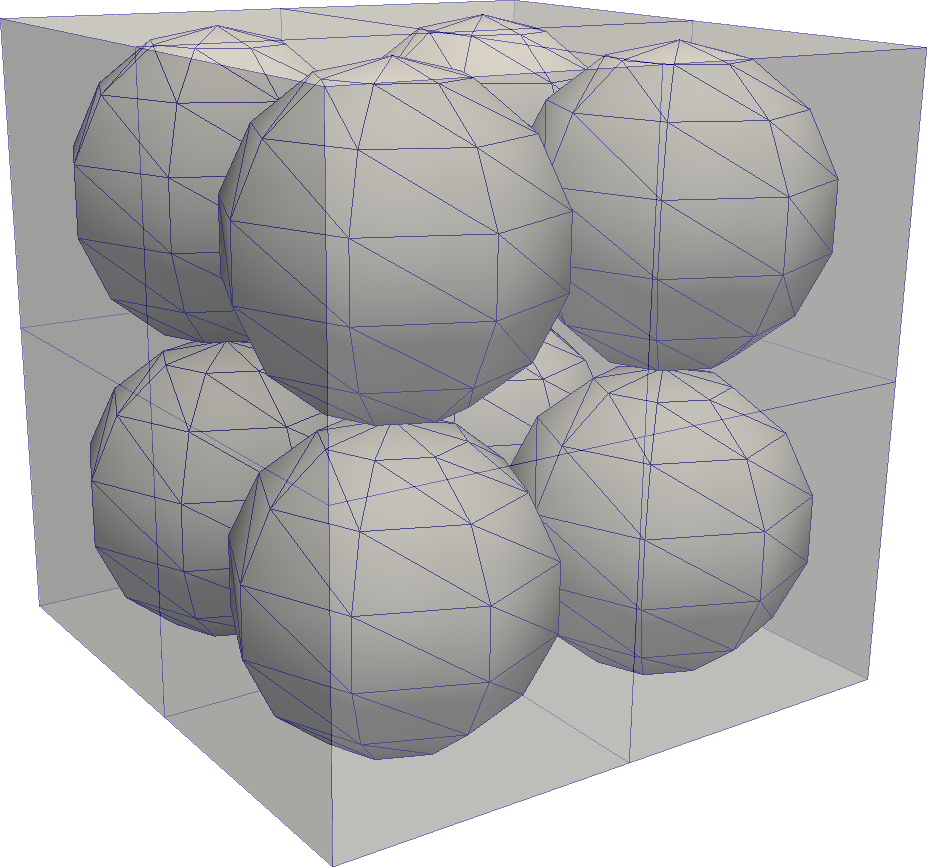
\includegraphics[width=0.85\linewidth]{Figures/ParaView/ParaView_Glyph_Mesh8}
    \caption{Resolution=8}
    \label{fig:ParaView_Glyph_Mesh8}
  \end{subfigure}%
  \begin{subfigure}{0.49\linewidth}
    \centering
    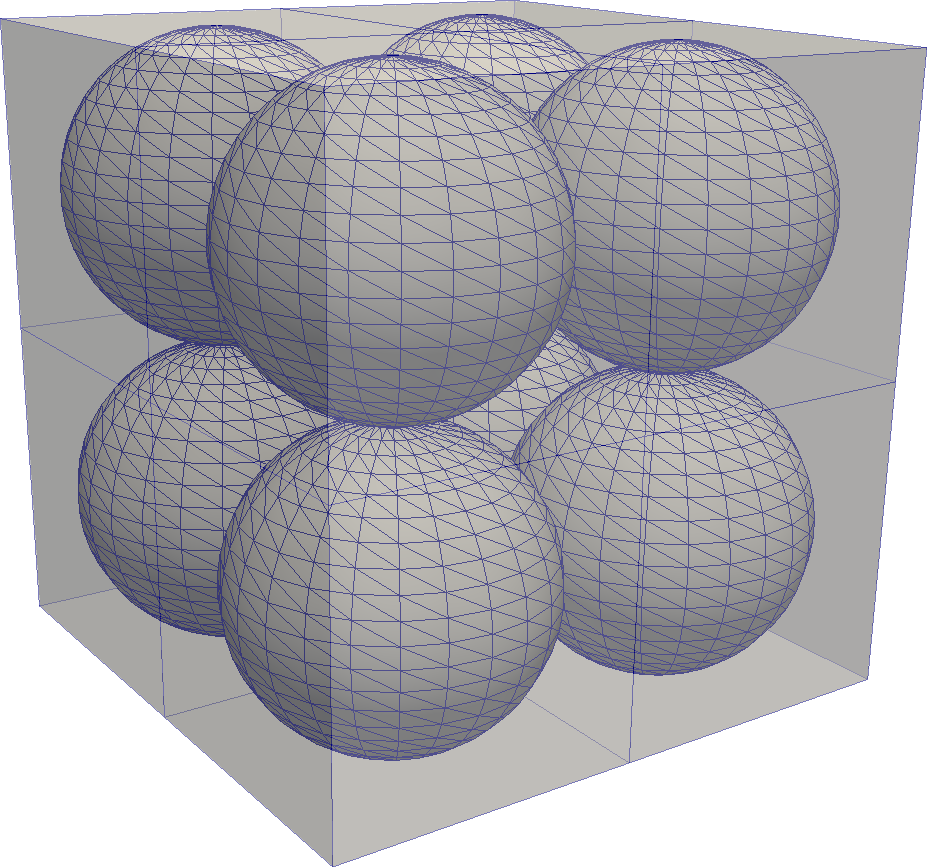
\includegraphics[width=0.85\linewidth]{Figures/ParaView/ParaView_Glyph_Mesh24}
    \caption{Resolution=24}
    \label{fig:ParaView_Glyph_Mesh24}
  \end{subfigure}%
  \caption{\protect\marktool{\toolname} collocation points inside the base finite element mesh with different glyph resolutions}
  \label{fig:ParaView_Glyph_Mesh}
\end{figure}



\newpage
%%%%%%%%%%%%%%%%%%%%%%%%%%%%%%%%%%%%
% Header                           %
%%%%%%%%%%%%%%%%%%%%%%%%%%%%%%%%%%%%
% 
% Revisions: 2017-04-10 Martin R�del <martin.raedel@dlr.de>
%                       Initial draft
%               
% Contact:   Martin R�del,  martin.raedel@dlr.de
%            DLR Composite Structures and Adaptive Systems
%          
%                                 __/|__
%                                /_/_/_/  
%            www.dlr.de/fa/en      |/ DLR
% 
%%%%%%%%%%%%%%%%%%%%%%%%%%%%%%%%%%%%
% Content                          %
%%%%%%%%%%%%%%%%%%%%%%%%%%%%%%%%%%%%

\levelup{Calculate}

%%%%%%%%%%%%%%%%%%%%%%%%%%%%%%%%%%%%
% Header                           %
%%%%%%%%%%%%%%%%%%%%%%%%%%%%%%%%%%%%
% 
% Revisions: 2017-04-10 Martin R�del <martin.raedel@dlr.de>
%                       Initial draft
%               
% Contact:   Martin R�del,  martin.raedel@dlr.de
%            DLR Composite Structures and Adaptive Systems
%          
%                                 __/|__
%                                /_/_/_/  
%            www.dlr.de/fa/en      |/ DLR
% 
%%%%%%%%%%%%%%%%%%%%%%%%%%%%%%%%%%%%
% Content                          %
%%%%%%%%%%%%%%%%%%%%%%%%%%%%%%%%%%%%

\leveldown{Cell center}
\label{sec:ParaView:Calculate:Cell:Center}

\begin{enumerate}[noitemsep]
\item Import your model and create a selection if only specific cell volumes are of interest.
\item Select the model or selection in the \textit{Pipeline Browser}
\item From the menu bar:
  \begin{itemize}[noitemsep]
  \item Click Filters
  \item Click Alphabetical
  \item Click \textit{Cell centers}
  \end{itemize}
\item In the \textit{Properties} tab
  \begin{itemize}[noitemsep]
    \item Select all blocks of interest in the \textit{Composite Data Set Index}
  \end{itemize}
\item Click \textit{Apply}
\item Open a new \textit{Spreadsheet View}
\item In the \textit{Showing} combobox select your \textit{Cell Center Filter Name} and \textit{Point Data} in the \textit{Attribute} combobox
\item Column \textit{points} shows the cell center
\end{enumerate}
%%%%%%%%%%%%%%%%%%%%%%%%%%%%%%%%%%%%
% Header                           %
%%%%%%%%%%%%%%%%%%%%%%%%%%%%%%%%%%%%
% 
% Revisions: 2017-04-10 Martin R�del <martin.raedel@dlr.de>
%                       Initial draft
%               
% Contact:   Martin R�del,  martin.raedel@dlr.de
%            DLR Composite Structures and Adaptive Systems
%          
%                                 __/|__
%                                /_/_/_/  
%            www.dlr.de/fa/en      |/ DLR
% 
%%%%%%%%%%%%%%%%%%%%%%%%%%%%%%%%%%%%
% Content                          %
%%%%%%%%%%%%%%%%%%%%%%%%%%%%%%%%%%%%

\levelstay{Cell volume}
\label{sec:ParaView:Calculate:Cell:Volume}

A method is described that allows the calculation/extraction of the cell or element volume. This solution is copied from the \href{https://public.kitware.com/pipermail/paraview/2015-October/035367.html}{Paraview Mailing List}.

\begin{enumerate}[noitemsep]
\item Import your model and create a selection if only specific cell volumes are of interest.
\item Select the model or selection in the \textit{Pipeline Browser}
\item From the menu bar:
  \begin{itemize}[noitemsep]
  \item Click Filters
  \item Click Data Analysis
  \item Click \textit{Programmable Filter}
  \end{itemize}
\item In the \textit{Properties} tab
  \begin{itemize}[noitemsep]
    \item Add to the \textit{Script} field:
\begin{code}
from vtk.numpy_interface import algorithms as algs

volume = algs.volume(inputs[0])
output.CellData.append(volume, 'volume')
\end{code}
    \item Select all blocks of interest in the \textit{Composite Data Set Index}
  \end{itemize}
\item Click \textit{Apply}
\item Open a new \textit{Spreadsheet View}
\item In the \textit{Showing} combobox select your \textit{Programmable Filter} and \textit{Cell Data} in the \textit{Attribute} combobox
\item Column \textit{volume} shows the cell volume
\end{enumerate}

\begin{figure}[htbp]
\centering
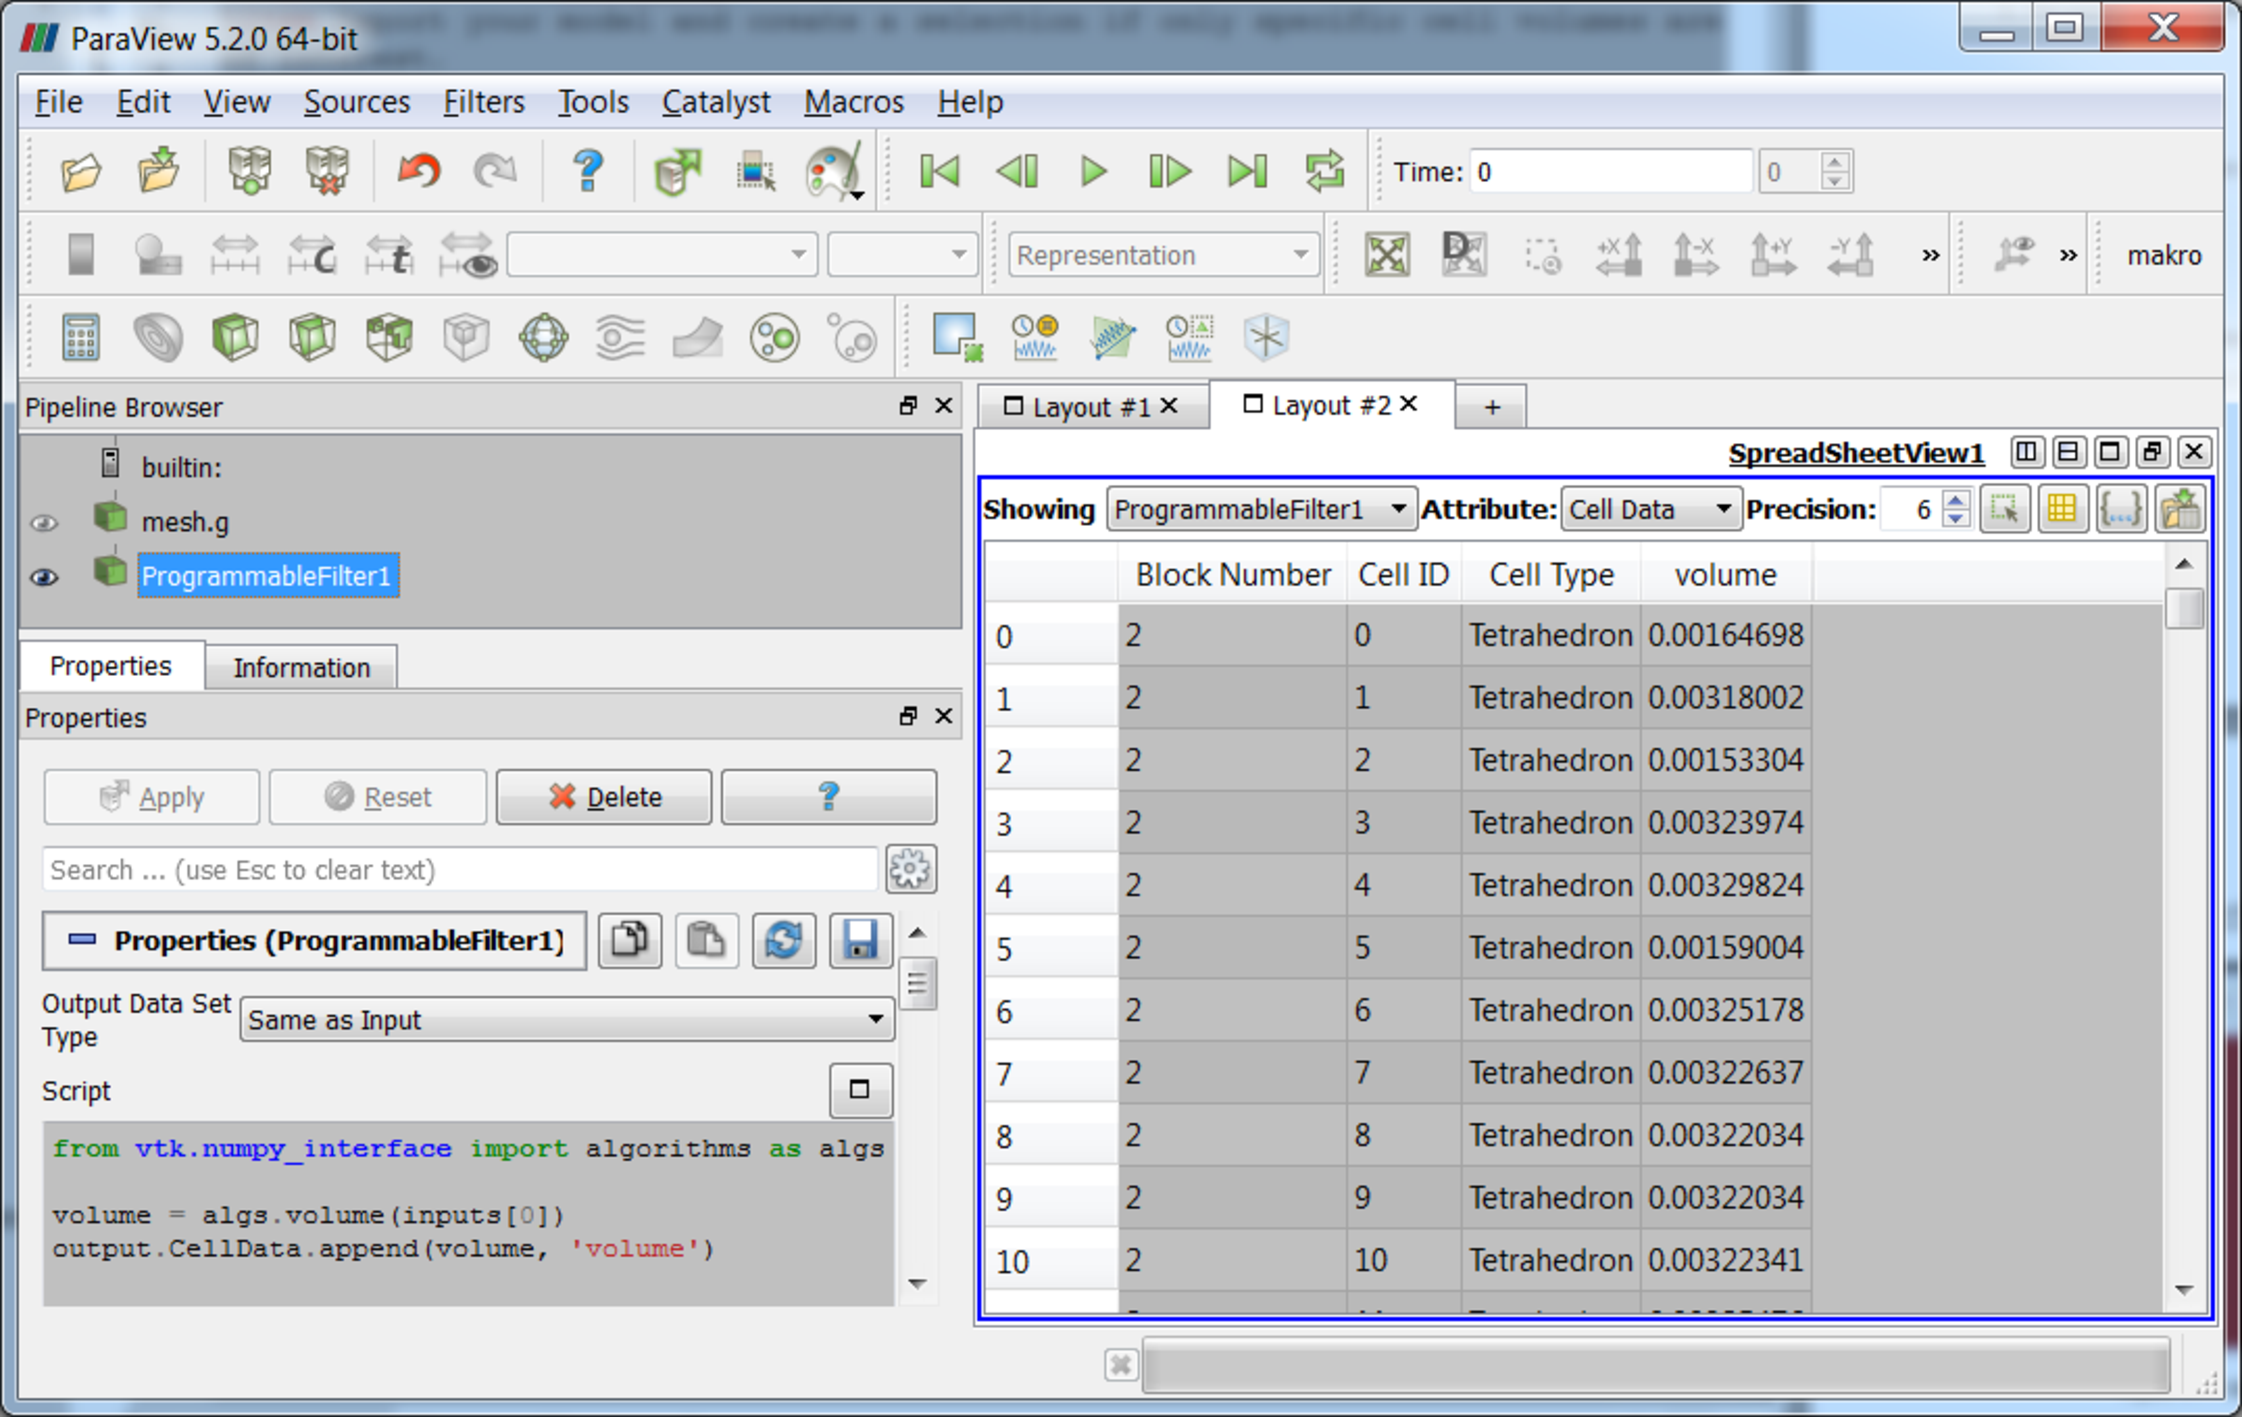
\includegraphics[width=\paraviewscreenshotwidthfac\linewidth]{Figures/Screenshots/ParaView_Calculate_Cell_Volume}
\caption{Display of cell volume calculation}
\label{fig:ParaView:Calculate:Cell:Volume}
\end{figure}
